

% \layout
%     \setlength{\hoffset}{0pt}
%     \setlength{\voffset}{0pt}
%     \setlength{\topmargin}{0pt}
%     \setlength{\oddsidemargin}{0pt}
%     \setlength{\marginparwidth}{0pt}
%     \setlength{\marginparsep}{0pt}
%     \setlength{\textwidth}{465pt}
%     \setlength{\textheight}{600pt}
% \layout*


\section{Supporting Information}

\begin{supplementary}

\subsection{ROSSpy}

The variables and terms that comprise our model are defined in Table \ref{glossary}.

\begin{longtable}{c|c|c}
    \caption{
        Glossary of ROSSpy variables.  
        \label{glossary} 
    } \\ \toprule
    
    \textbf{variable} & \textbf{name} & \textbf{description} \\ \toprule
    \endfirsthead
    \multicolumn{3}{c}{continuation of Table \ref{glossary}} \\  \toprule
    \textbf{variable} & \textbf{name} & \textbf{description} \\ \toprule
    \endhead
    
    \multirow{2}{1.5em}{$l$} & \multirow{2}{3em}{length} & longitudinal dimension of the\\& & module or module cell \\ \midrule
    \multirow{2}{1.5em}{$n$} & number of & quantity of discretizations of the module \\ & module cells & \\ \midrule
    $\Phi_e$ & moles & the $moles_{H_2O}$ that exist in cell $e$ \\ \midrule  
    $\Delta \Phi_e$ & permeate flux & the $moles_{H_2O}$ that are removed in cell $e$ \\ \midrule  
    $HL$ & head loss & reduction of pressure over the module distance \\ \midrule
    \multirow{2}{2em}{$PE$} & \multirow{2}{3em}{permeate efficiecy} & attenuation of permeate flux \\& & from pre-existing inefficiencies \\ \midrule  
    \multirow{2}{2em}{$CF$} & \multirow{2}{3em}{concentration factor} & solution concentration of cell $e$ normalized \\& & to the influent concentration \\ \midrule
    $X$ & mass & water mass in the maximally filled feed channel \\ \midrule
    $V$ & velocity & feed velocity through the feed channel \\ \midrule
    $A$ & area & cross-sectional area of the RO module \\ \midrule
    $th$ & thickness & thickness of a module dimension \\ \midrule
    $Q$ & volumetric flow & feed flow through a maximally filled feed channel \\ \midrule
    \multirow{2}{1.5em}{$\Delta t$} & \multirow{2}{3em}{time} & timestep of the simulation that \\& & adheres to the Courant condition \\ \midrule
    \multirow{2}{2em}{$C_{max}$} & \multirow{2}{3em}{Courant constant} & maximal value of the Courant constant \\& & to meet the Courant condition \\ \midrule
    $\phi$ & total concentration & total ionic concentrations in the simulation \\ \midrule
    $C$ & specie concentration & concentration of an individual specie \\ \midrule
    \multirow{2}{1em}{$v$} & \multirow{2}{3em}{stoichiometry coefficient} & coefficient for the respective compound \\& & in the balanced equilibrium reaction \\ \midrule
    \multirow{2}{1em}{$N$} & number of & quantity of reactions that \\& reactions & contain a respective compound \\ \midrule
    $R$ & reaction flux & $\frac{mmol}{hour}$ flux of an equilibrium reaction \\ \midrule
    \multirow{2}{1em}{$\Omega$} & thermodynamic & logarithm of the $\frac{Q_{dissolution}}{K_{sp}}$ \\& displacement & \\ \midrule
    $k_m$ & rate constant & dissolution and precipitation rate constant \\ \midrule
    $a$ & activity & chemical activity of the respective compound \\ \midrule
    $\eta$ \& $p$ & parameter & experimentally determined parameter \\ \midrule
    \multirow{2}{2em}{$\Delta G$} & \multirow{2}{5em}{Gibbs free energy} & Gibbs free energy of the dissolution \\& & and precipitation reactions \\ \midrule
    $K$ & equilibrium constant & thermodynamic equilibrium of the respective reaction \\ \midrule
    $M$ & number of minerals & quantity of minerals in the studied system \\ \midrule
    $\gamma$ & activity coefficient & coefficient of metabolite activity in a respective system \\ \midrule
    $z$ & charge & compound charge of the respective metabolite \\ \midrule
    $\mu$ & ionic strength & charge-weighted concentration of a solution \\ \midrule
    $A$ \& $B$ & parameter & experimentally determined parameter \\ \midrule
    $a_j$ \& $b_j$ & fitted parameter & geochemical parameter that is fit to the system \\ \midrule
    $W_{aq}$ & water mass & mass of water in the system \\ \bottomrule
\end{longtable} 

The distinctions between slicing the simulation data through time or module distance is exhibited with brine in Figure \ref{brine_perspectives} and scaling in Figure \ref{scaling_perspectives}, respectively.

\begin{figure}
    \centering
    \begin{tabular}{c}
        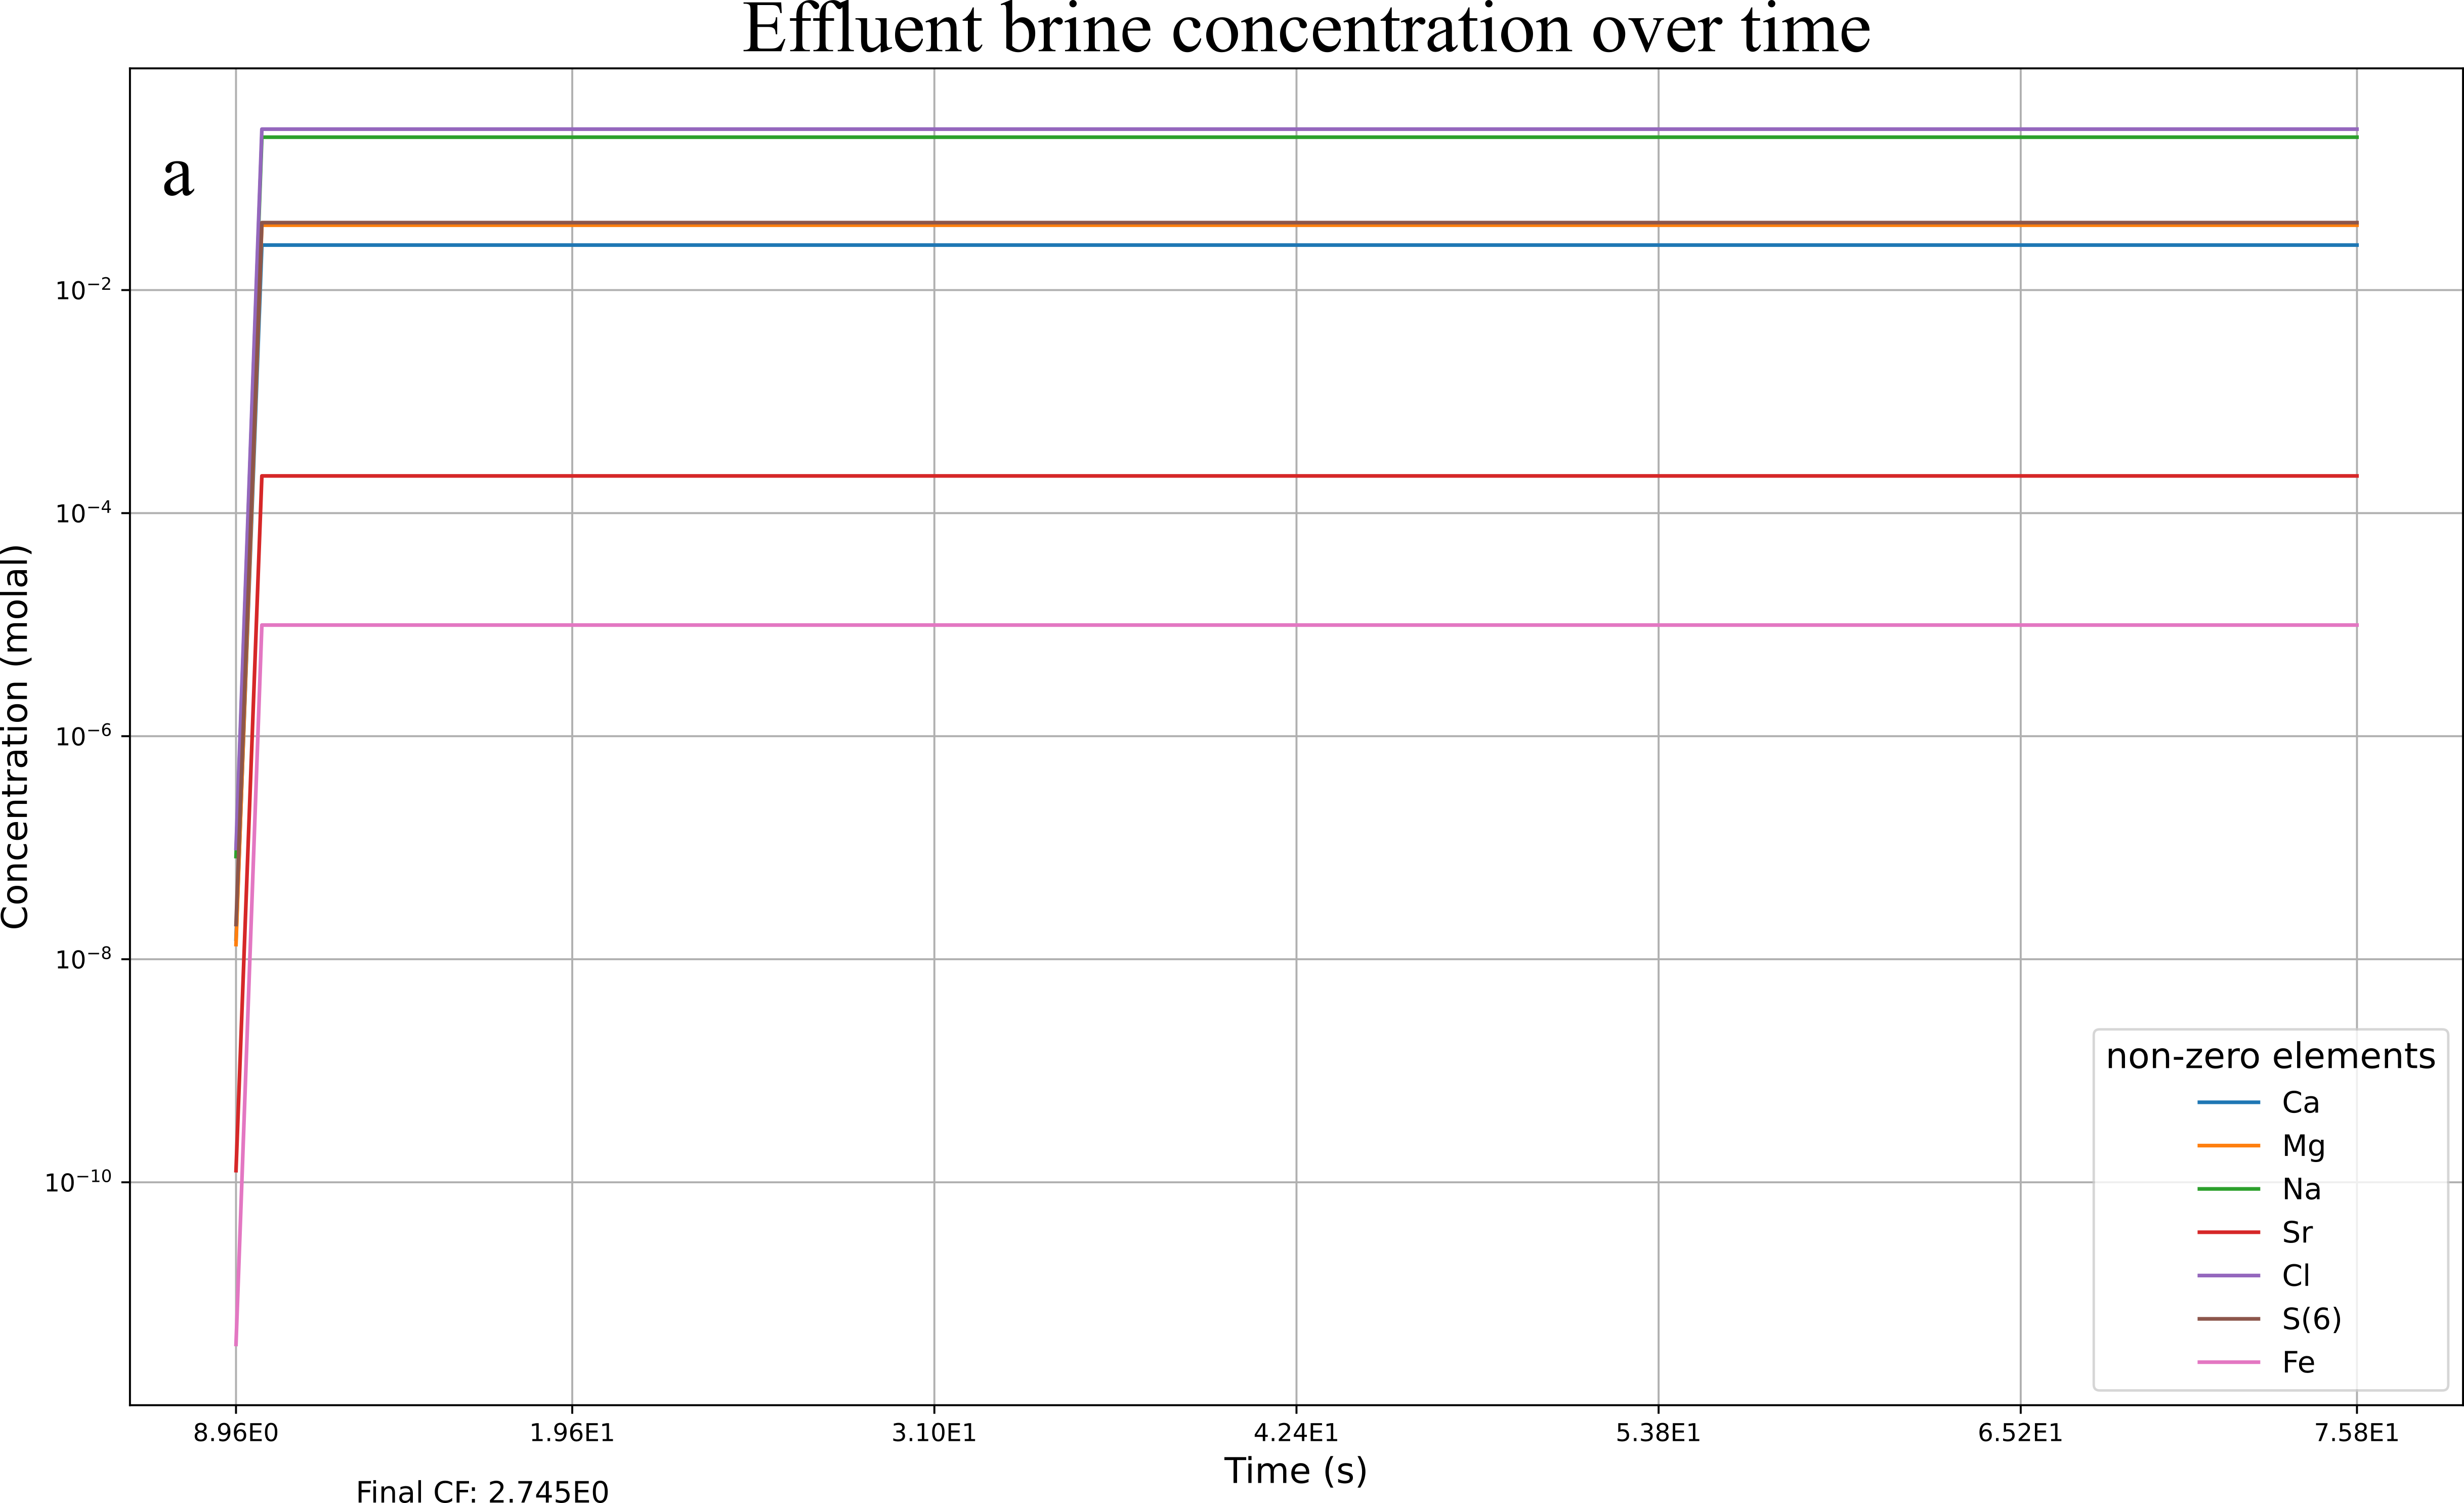
\includegraphics[width=0.8\linewidth]{images/ROSSpy/sensitivity_analyses/simulation_perspective/all_time_brine.png} \\ \midrule
        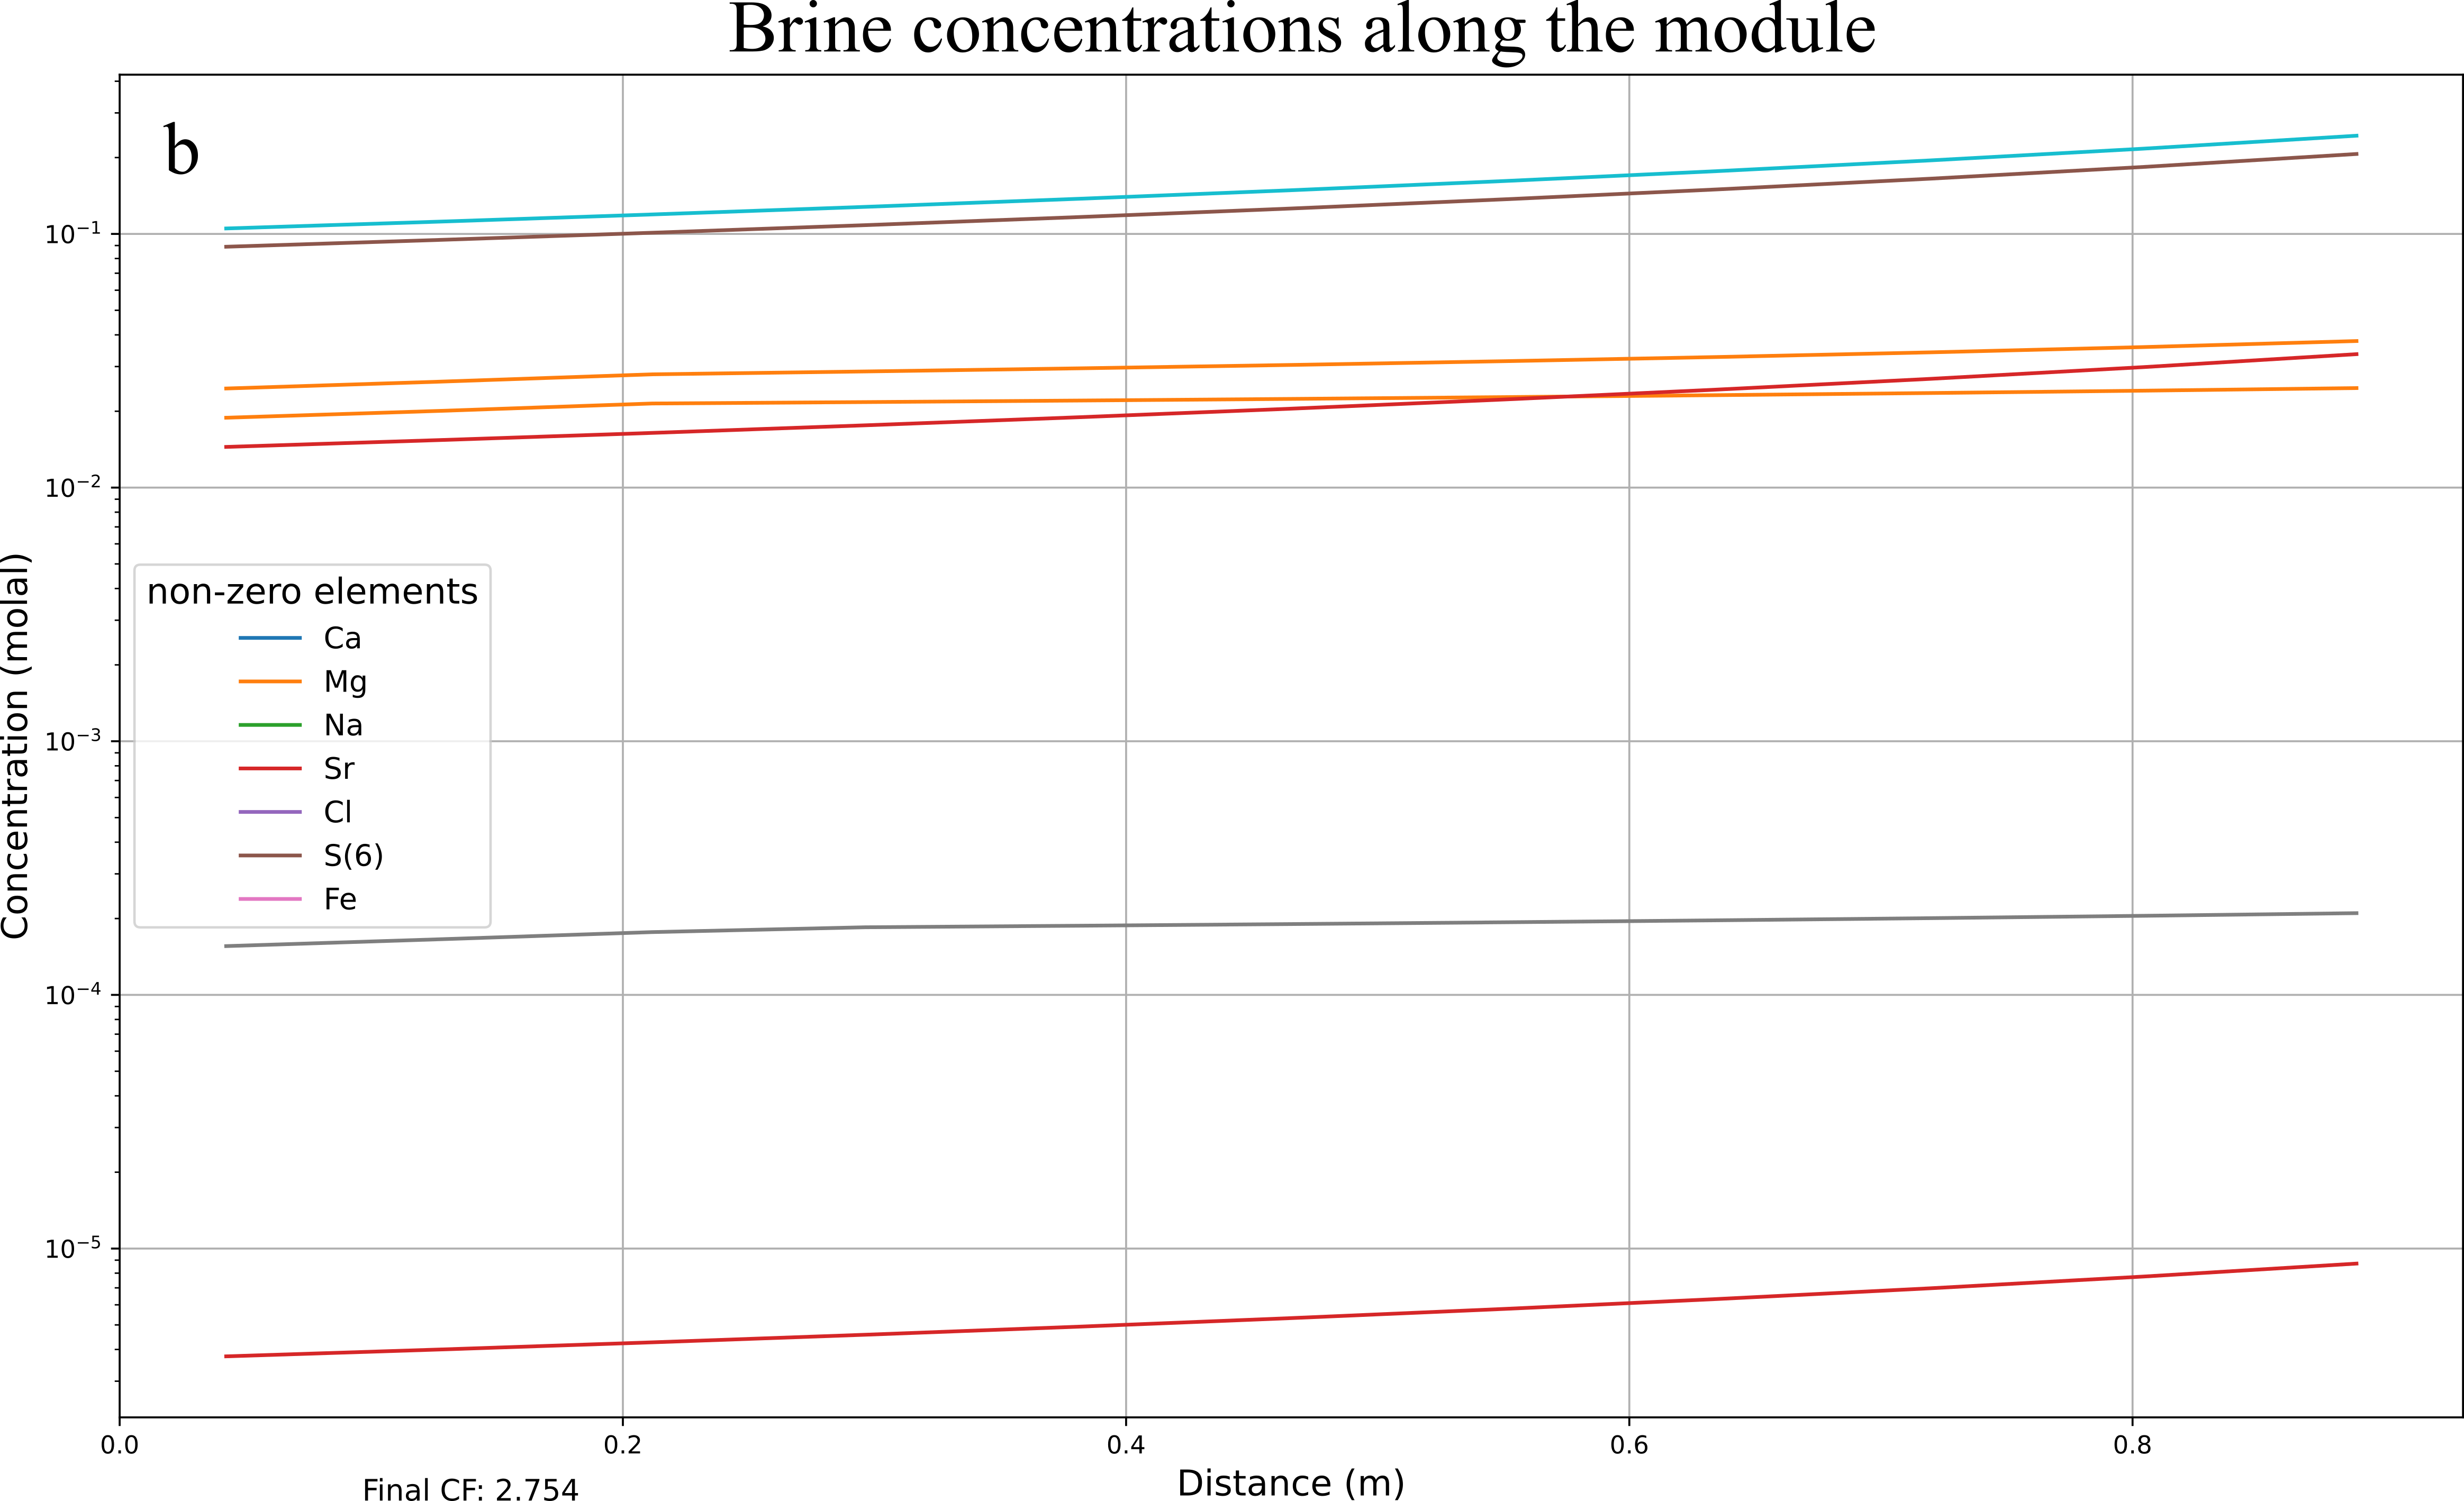
\includegraphics[width=0.8\linewidth]{images/ROSSpy/sensitivity_analyses/simulation_perspective/all_distance_brine.png}
    \end{tabular}
    \caption{
        Brine formation while slicing through either a) time at the final cell or b) distance at the final time. The end concentrations slightly differ between these two simulation perspectives, where the all\_time perspective calculates the true end of the last cell while the all\_distance perspective calculates the mid-point of the last cell and thus has a slightly lower concentration. The brine represents desalination of the Red Sea through the BW30-400 module.
    }
    \label{brine_perspectives}
\end{figure}

\begin{figure}
    \centering
    \begin{tabular}{c}
        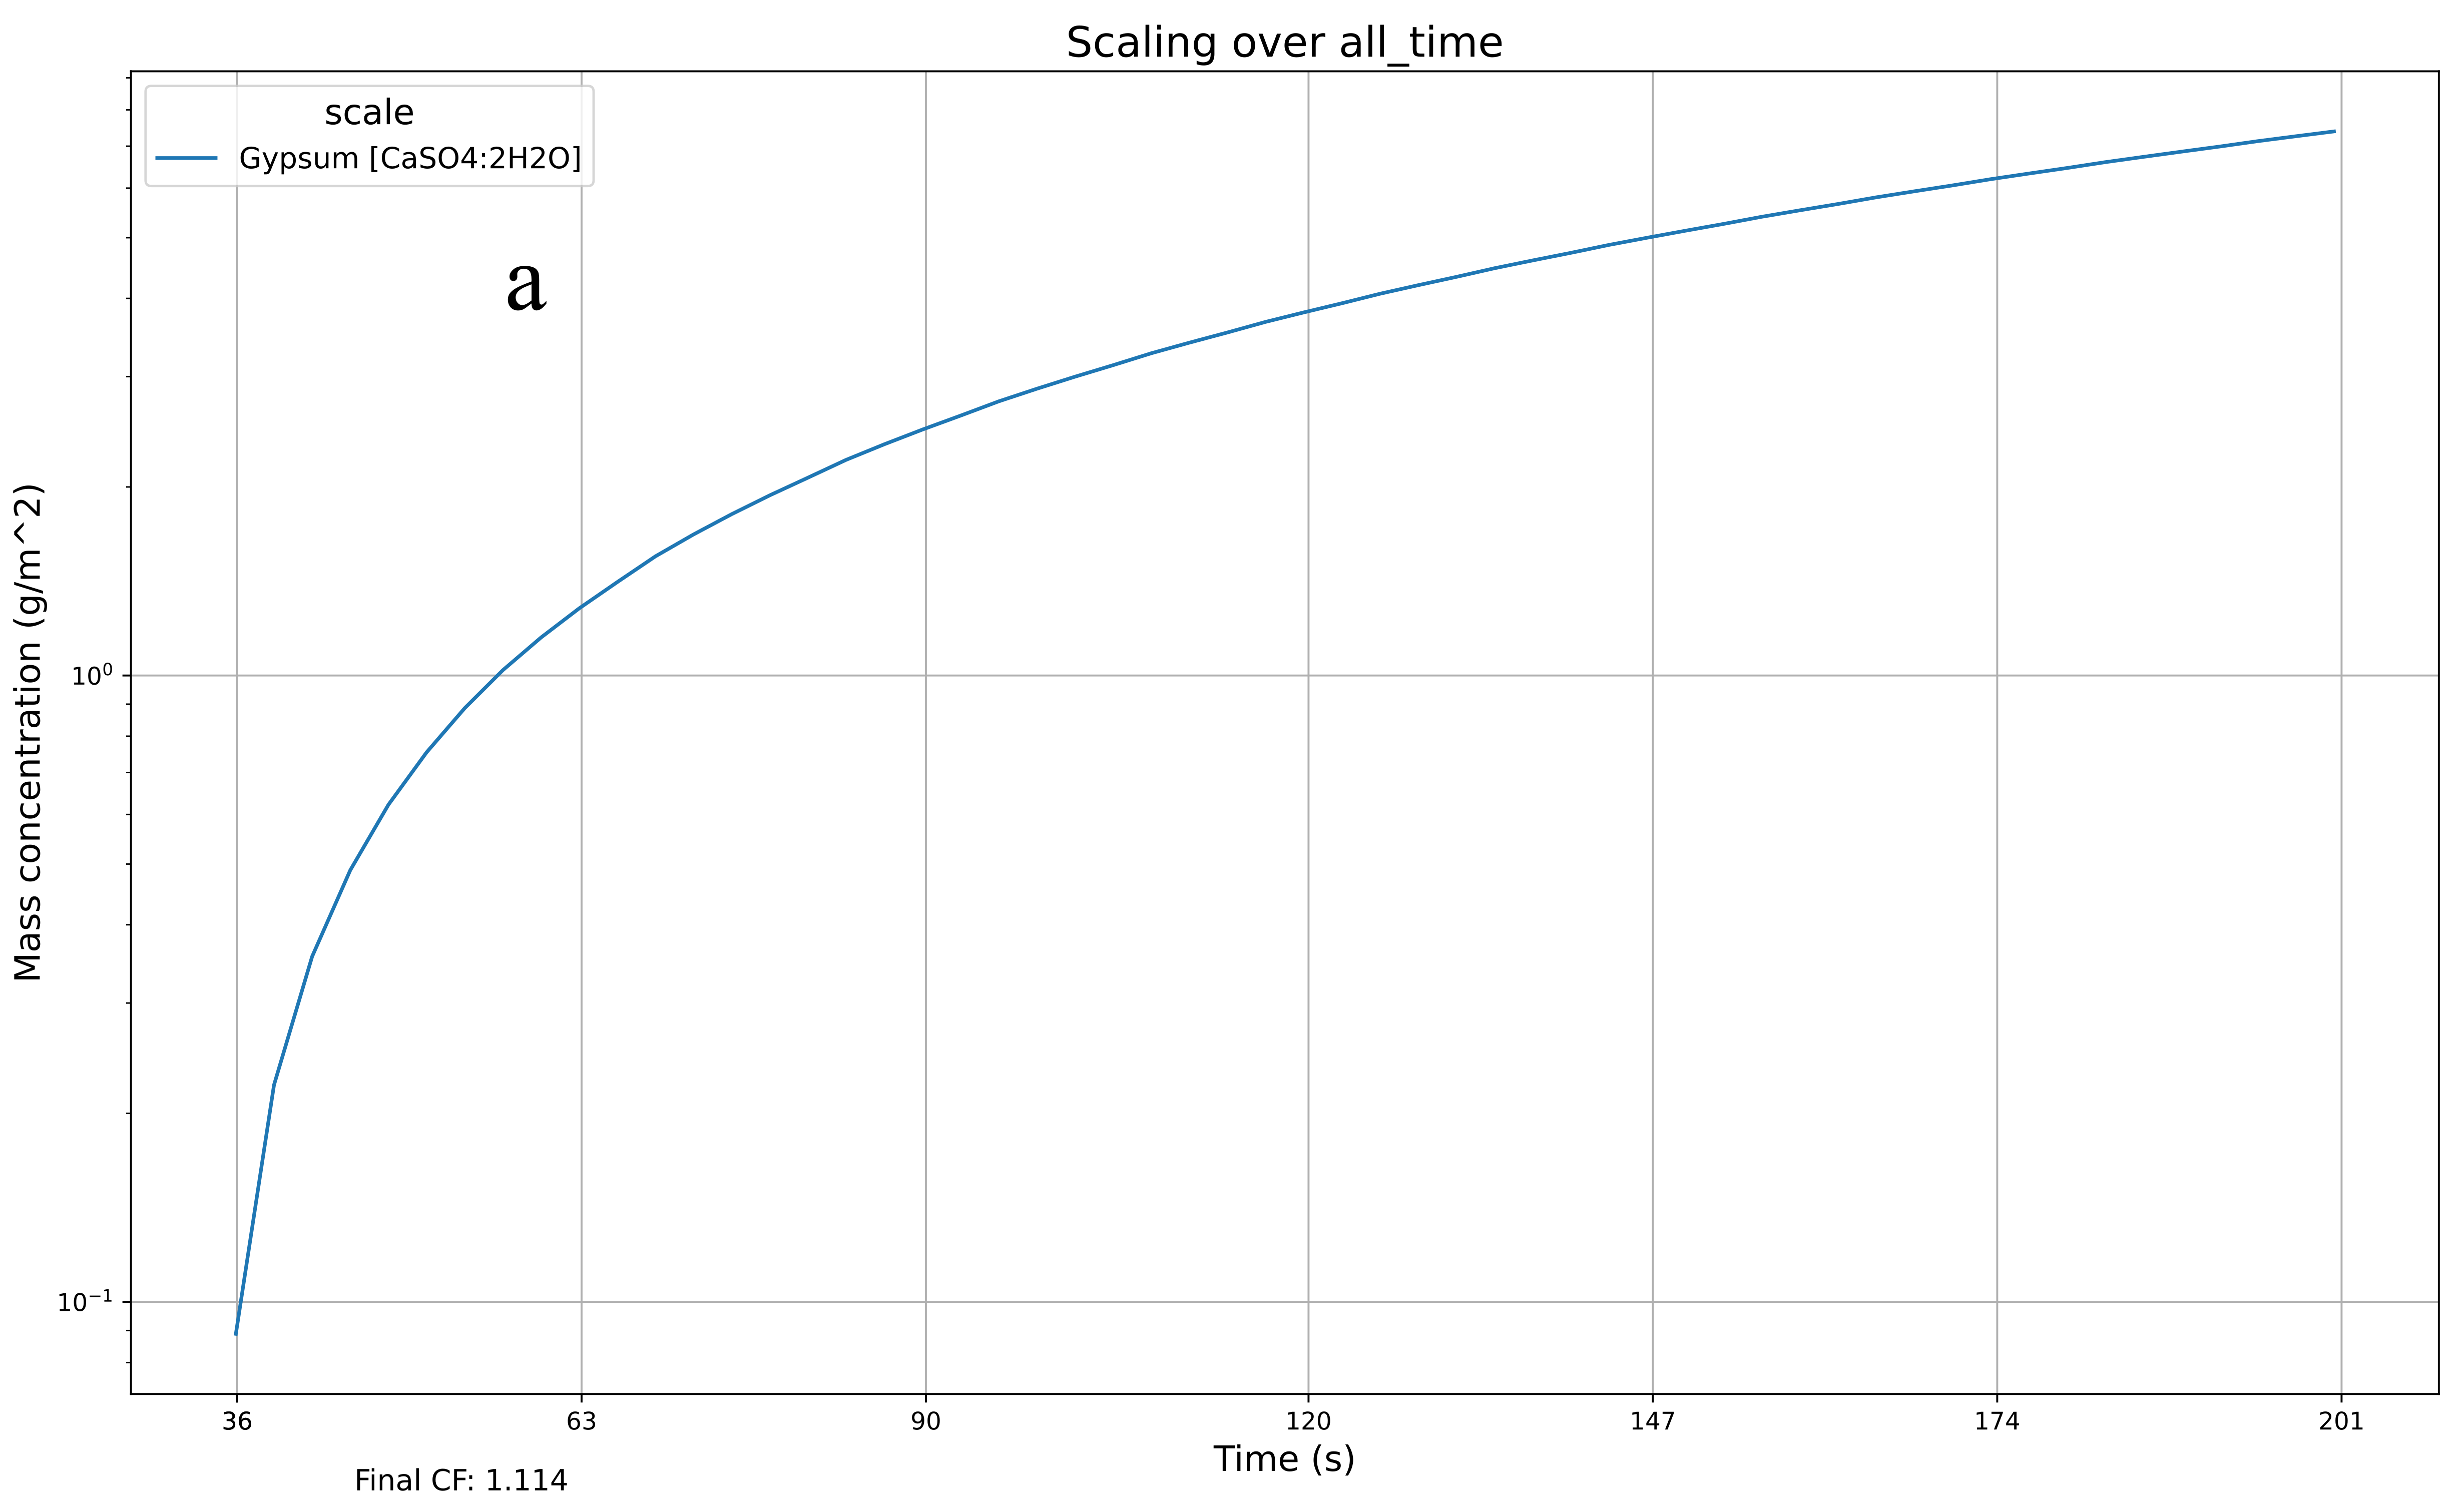
\includegraphics[width=\linewidth]{images/ROSSpy/sensitivity_analyses/simulation_perspective/all_time.png} 
        \\ \midrule
        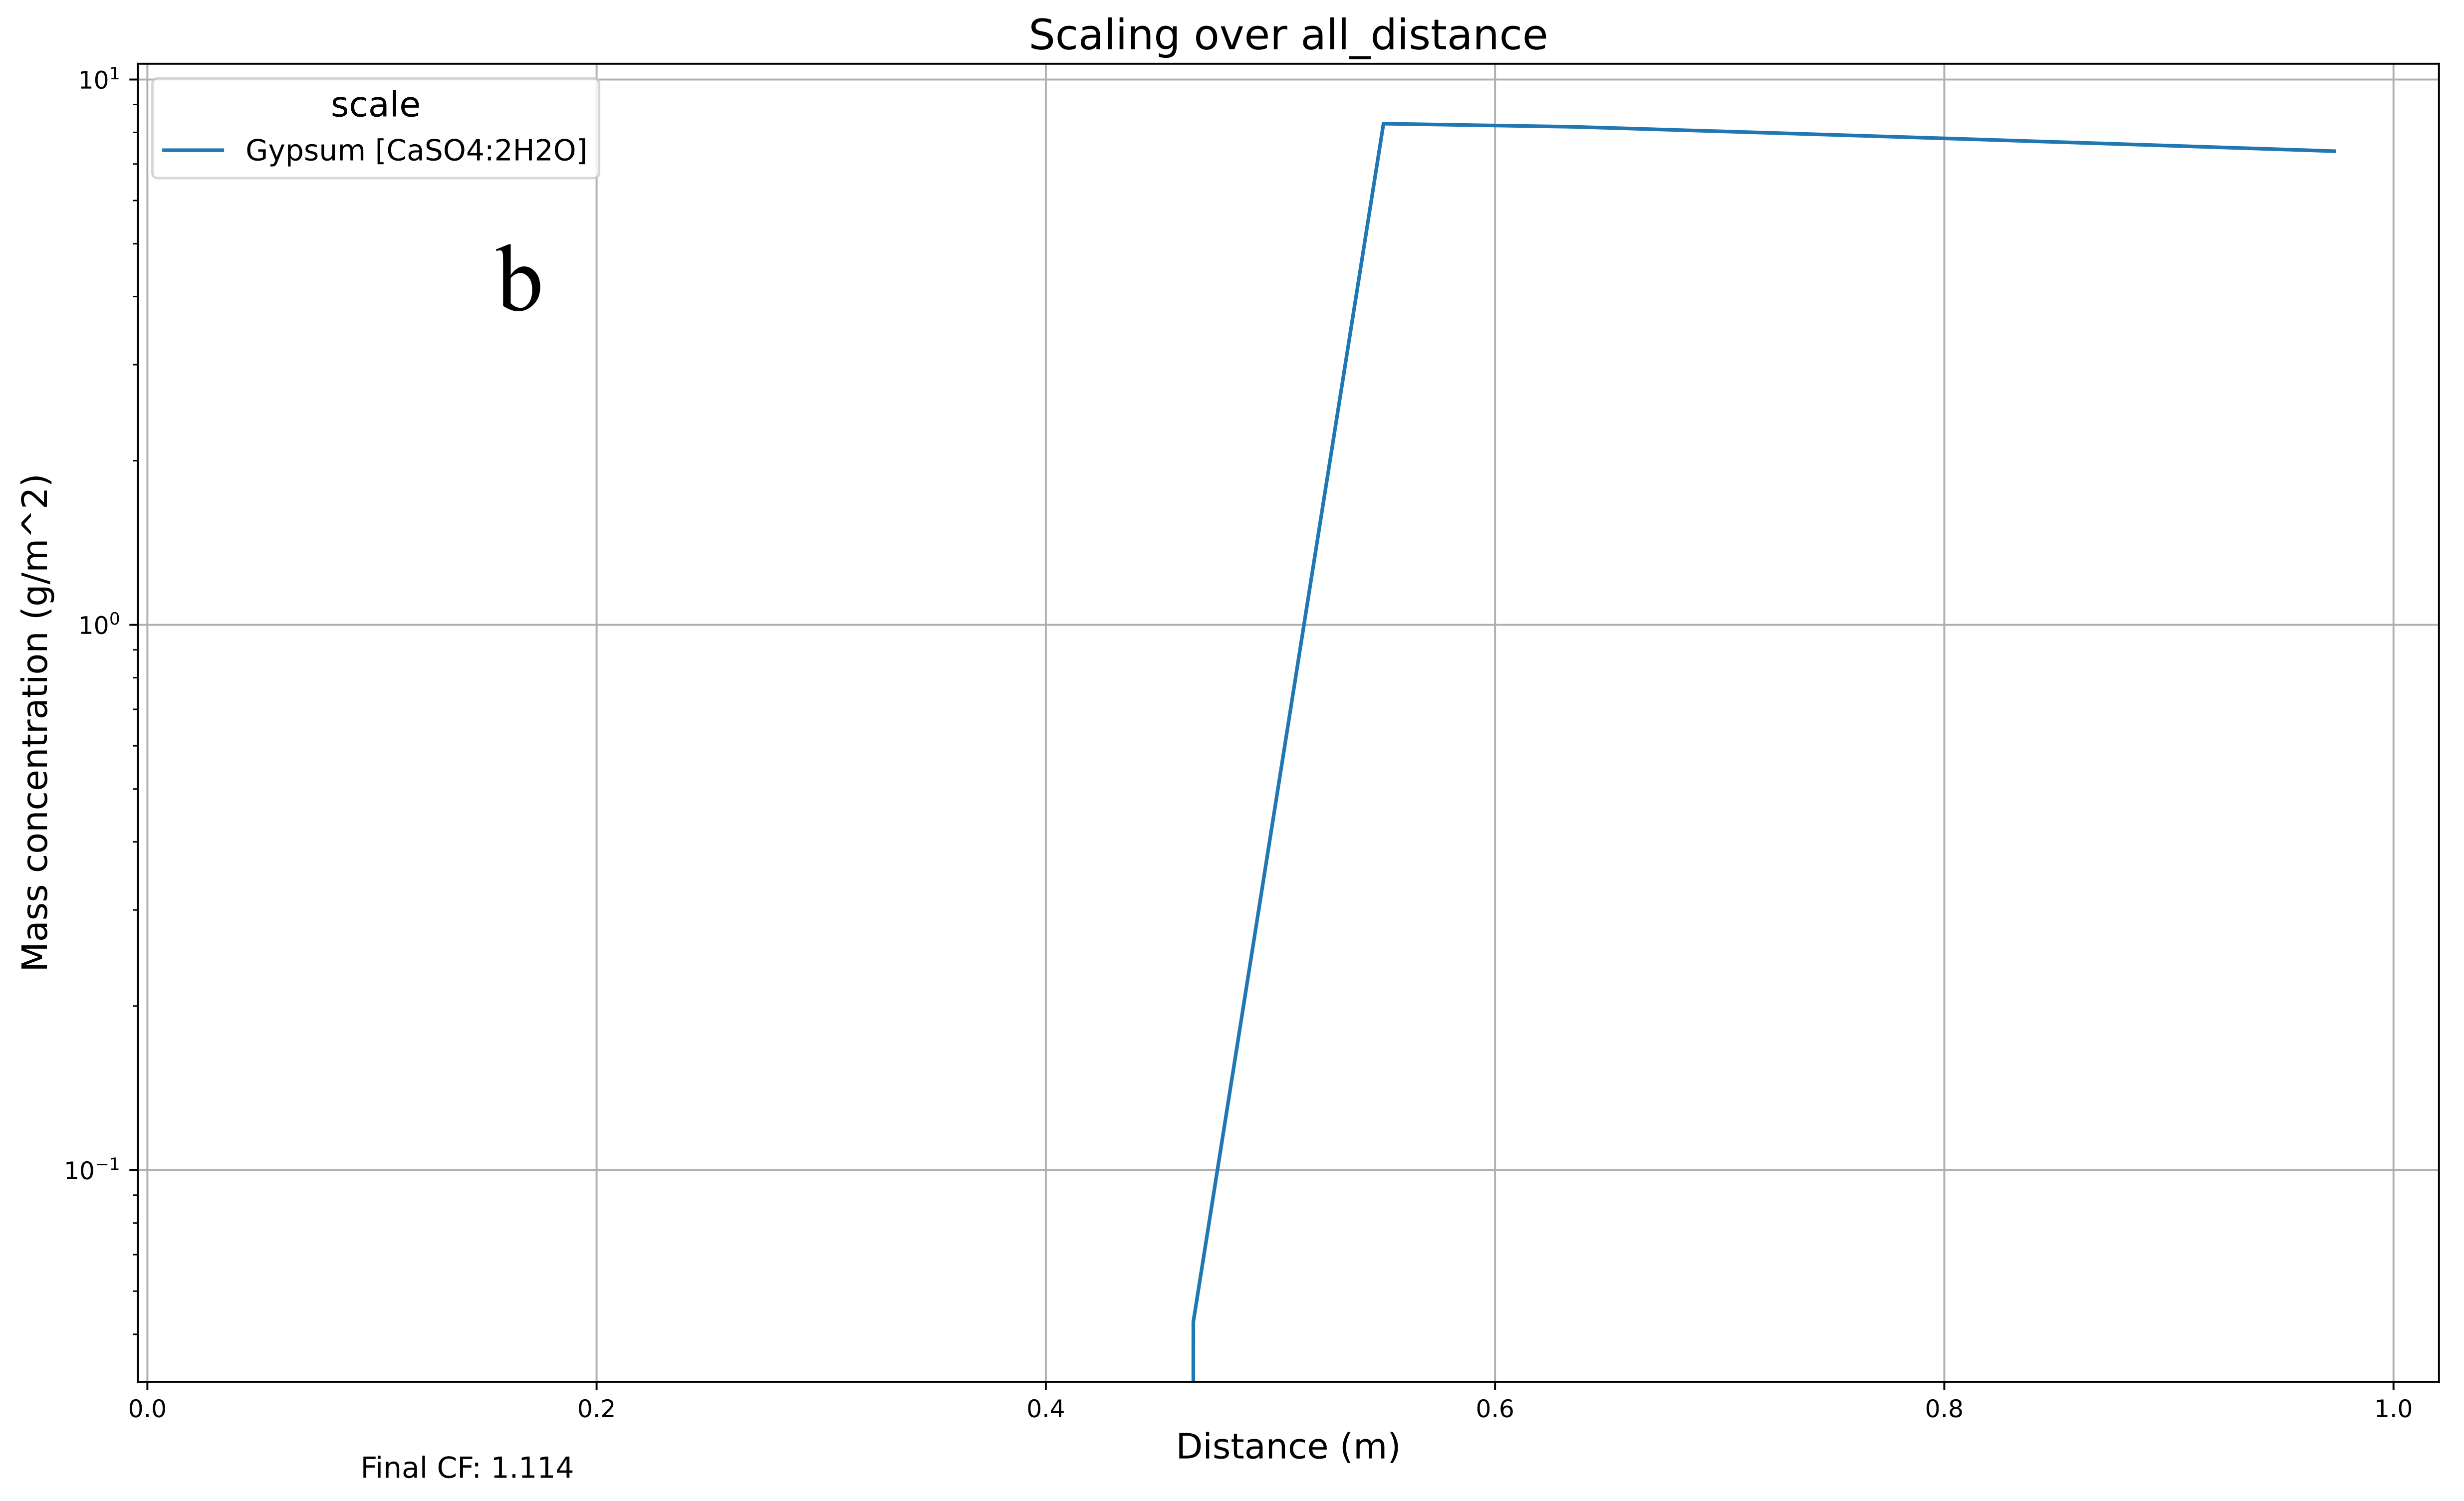
\includegraphics[width=\linewidth]{images/ROSSpy/sensitivity_analyses/simulation_perspective/all_distance.png} 
    \end{tabular}
    \caption{
        Scaling while either slicing through a) time at the final cell or b) distance at the final time. The underlying simulation was of the Red Sea through the BW30-400 module.
    }
    \label{scaling_perspectives}
\end{figure}

A cross-section of an RO module, which highlights boundaries of the single- and dual-domain solution models, is depicted in Figures \ref{single_dual_domain}.

\subsection{Software}

\subsection{PHREEQC consistency}

\subsubsection{ICE table calculations}
The expected precipitation in the presented ICE table of Table \ref{ice_table} was determined as $x$ in the following derivation:

\begin{equation} \label{ice_calculations}
    \begin{split}
        K_{sp} &= [a_{Ca^{2+}} - x]^1 * [a_{SO_4^{2-}} - x]^1 \\ 
        K_{sp} &= (\gamma*[Ca^{2+}] - x) * (\gamma*[SO_4^{2-}] - x) \\ 
        10^{-4.58} &= ((0.19*0.020594) - x) * ((0.06*0.105462) - x) \\ 
        10^{-4.58} &= (0.003913 - x) * (0.00633 - x) \\
        10^{-4.58} &= 2.477E-5 - 0.01024 + X^2 \\
        0 &= -1.54E-6 - 0.01022x + x^2 \\
         \therefore ~~ x &= 0.0104~molal = \frac{\fbox{0.181~moles}}{17.67~kg~water}~~.
    \end{split}
\end{equation}

The activity coefficients ($\gamma$) for $Ca^{2+}$ and $SO_4^{2-}$ were sourced from PHREEQC for this specific solution system. The $17.67~kg$ mass of water corresponds to the mass maximum capacity of the simulated BW30-400 module.  

The predicted precipitation in the presented ICE table of Table 1b ($gypsum\_pore\_volume$) are similarly derived:
\begin{equation} \label{PHREEQC_output_precipitation}
    \begin{split}
        gypsum\_pore\_volume &= gypsum\_all\_shifts * \frac{cells\_per\_module}{total\_simulation\_shifts} \\
         &= \sum_{i=1}^n (Gypsum_i) * \frac{12}{51} \\ 
         &= 0.823 * \frac{12}{51} \\ 
         &= 0.194 ~moles ~~.
    \end{split}
\end{equation}
The $\frac{12}{51}$ is the fraction of simulation shifts that correspond to a single module or pore volume, where the simulated module was discritized into $12$ cells. This isolates scaling from a single module, instead of the accumulation of scaling from multiple pore volumes, which renders the quantity directly comparable with the expected quantity.

\begin{table}[h]
    \centering
    \begin{tabular}{c|ccccc}
      \toprule
       & $Ca^{2+}$ & $+$ & $SO_4^{2-}$ & $\leftrightharpoons$ & $CaSO_4$ \\
      \midrule
      I & $0.003913$ && $0.00633$ && $0$ \\
      C & $-x$ && $-x$ && $+x$ \\
      F & $0.003913-x$ && $0.00633-x$ && $x$ \\
      \bottomrule
    \end{tabular}
    \caption{
        Gypsum precipitation according to the ICE (Initial, Change, Equilibrium) framework, except that "Equilibrium" (E) is replaced with "Final" (F) since the system does not reach equilibrium while within the module. The estimated Gypsum precipitation from a solution of $Ca^{2+}$ \& $SO_4^{2-}$ -- based upon the $K_{sp}$ of Gypsum and the activity coefficients of this solution from iPHREEQC -- is derived in \ref{ice_calculations} for the system in this table. 
        }
    \label{ice_table}
\end{table}

\subsubsection{Evaporation versus transport desalination}

The mechanism of concentrating a solution, either via evaporation or desalination, should not alter scaling predictions, ceterius paribus. Figure \ref{evaporation} contrasts scaling predictions from evaporation and desalination of the Red Sea, where the two mechanisms are approximately equivalent. Differences are postulated to originate from the consideration of advection in the latter but not the former.

\begin{figure}
    \centering
    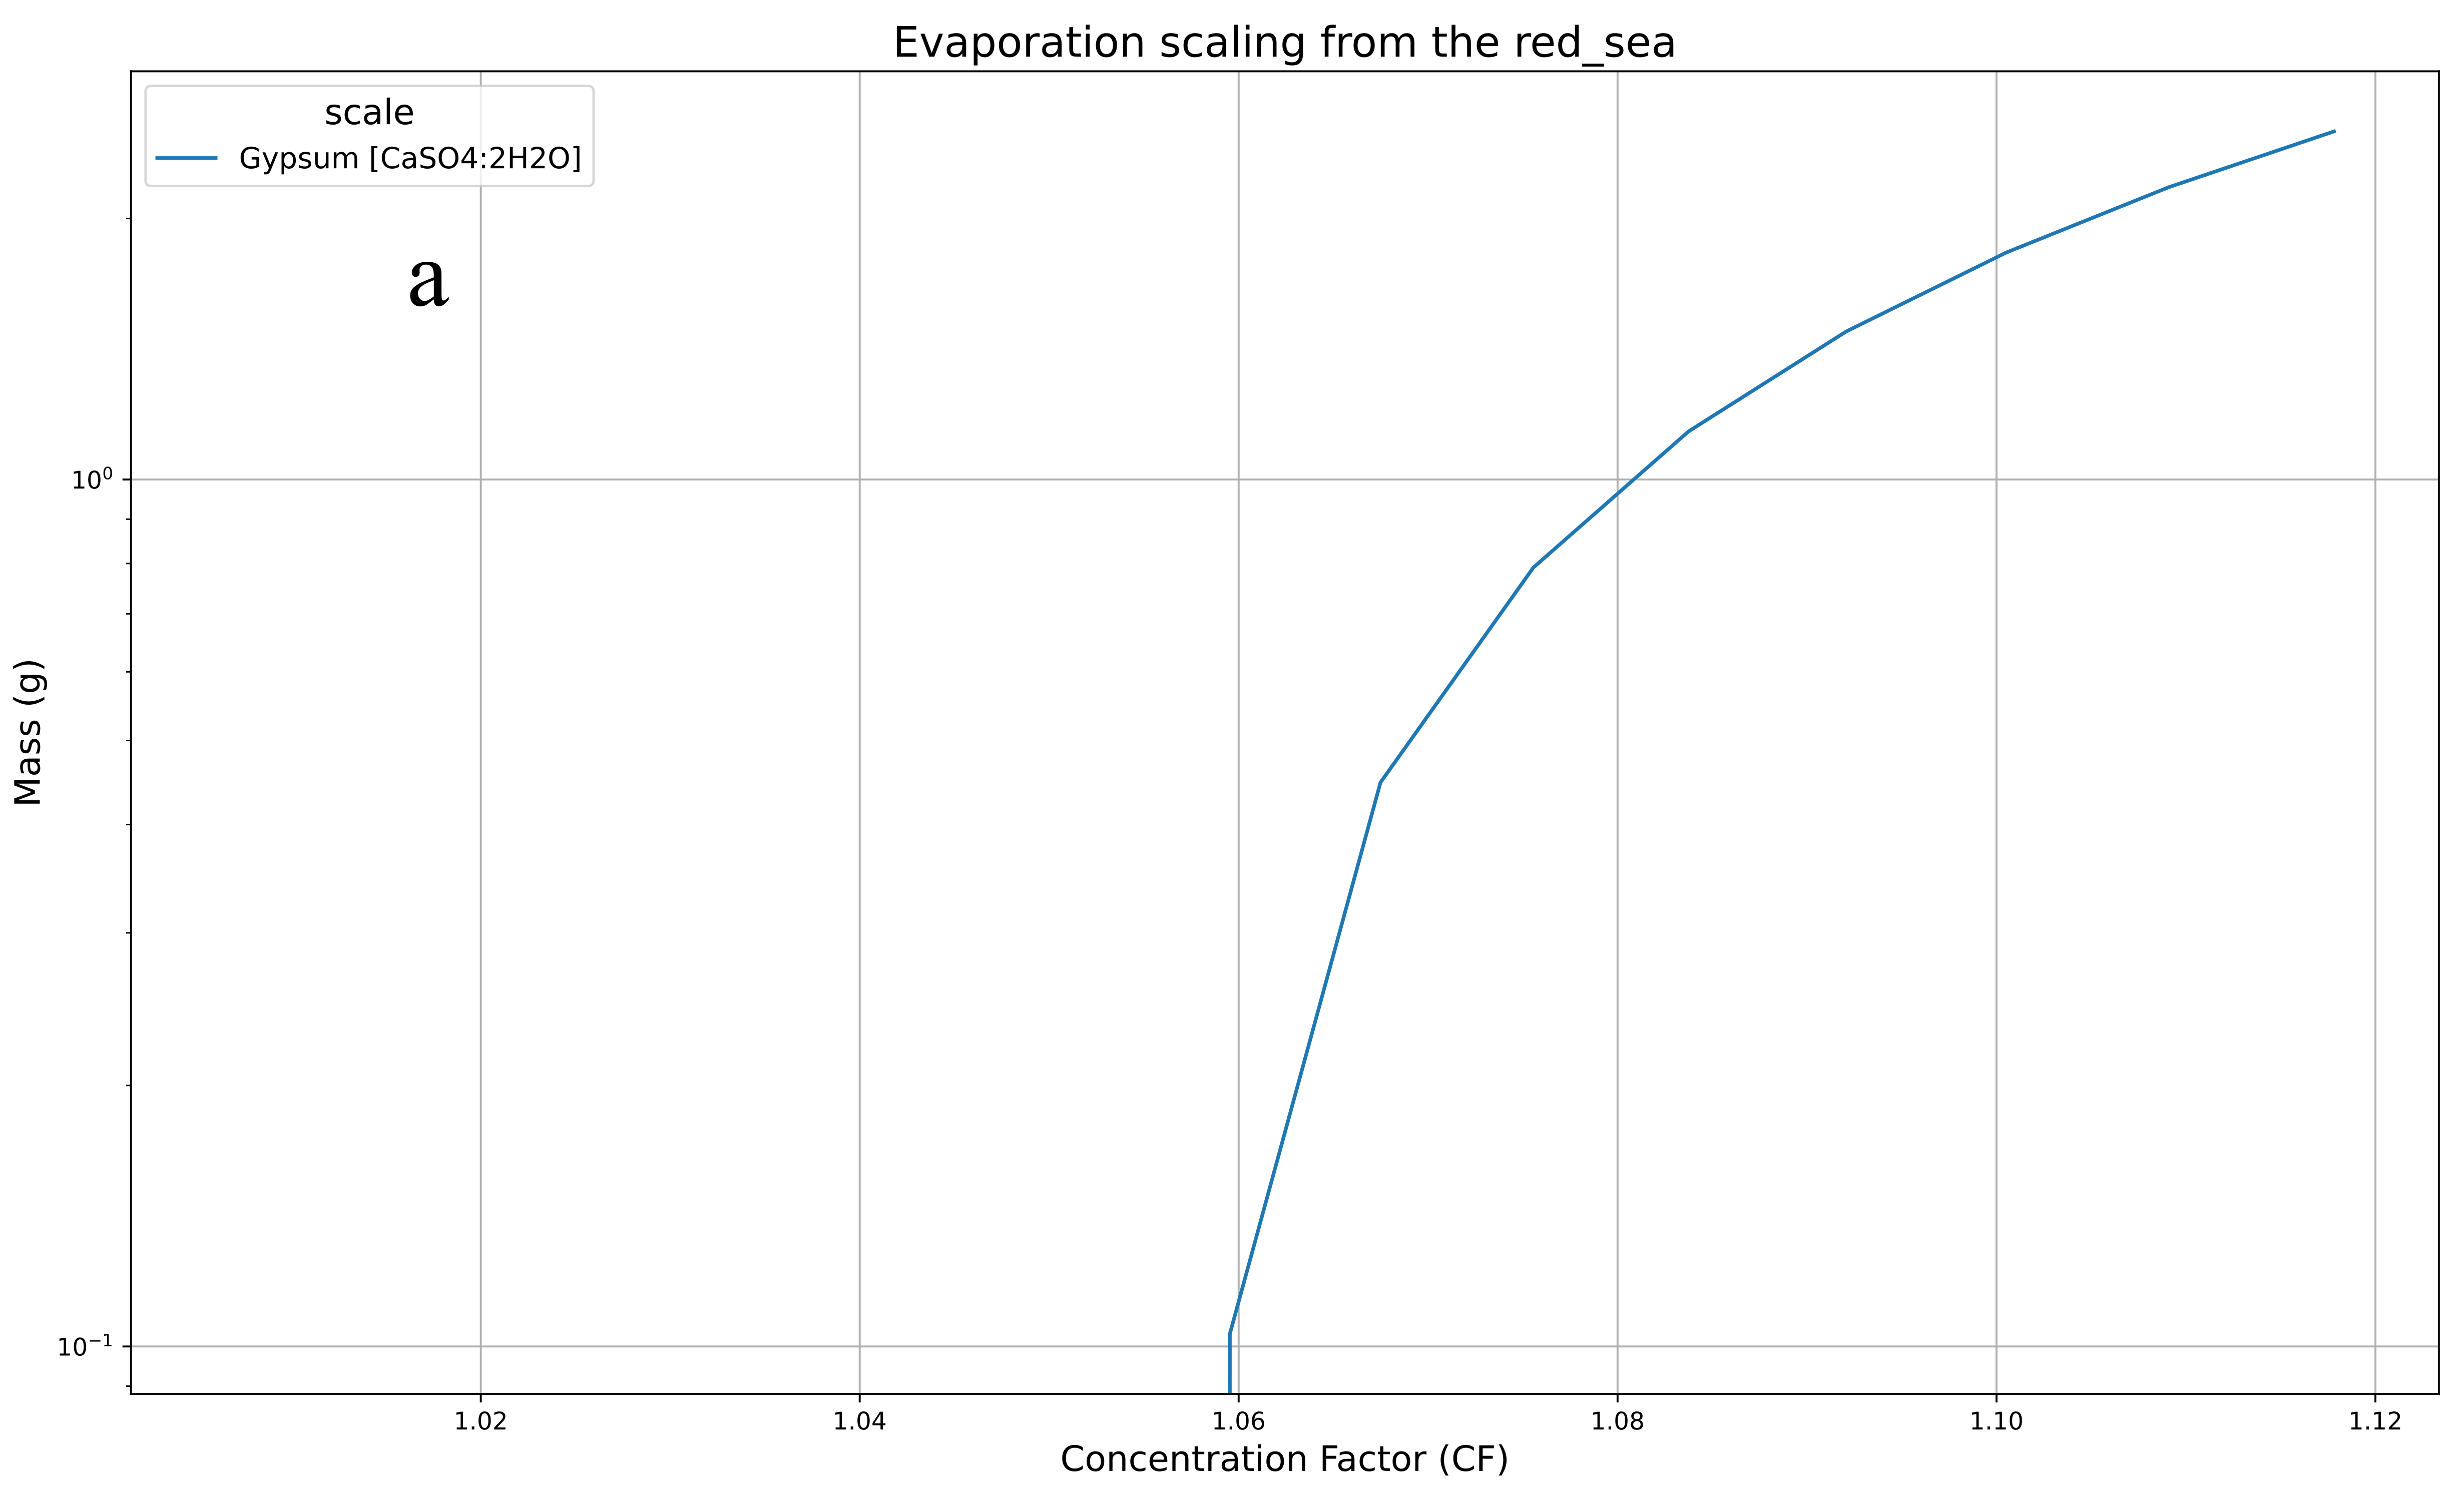
\includegraphics[width=\linewidth]{images/ROSSpy/sensitivity_analyses/evaporation/evaporation.png} \\ \midrule
    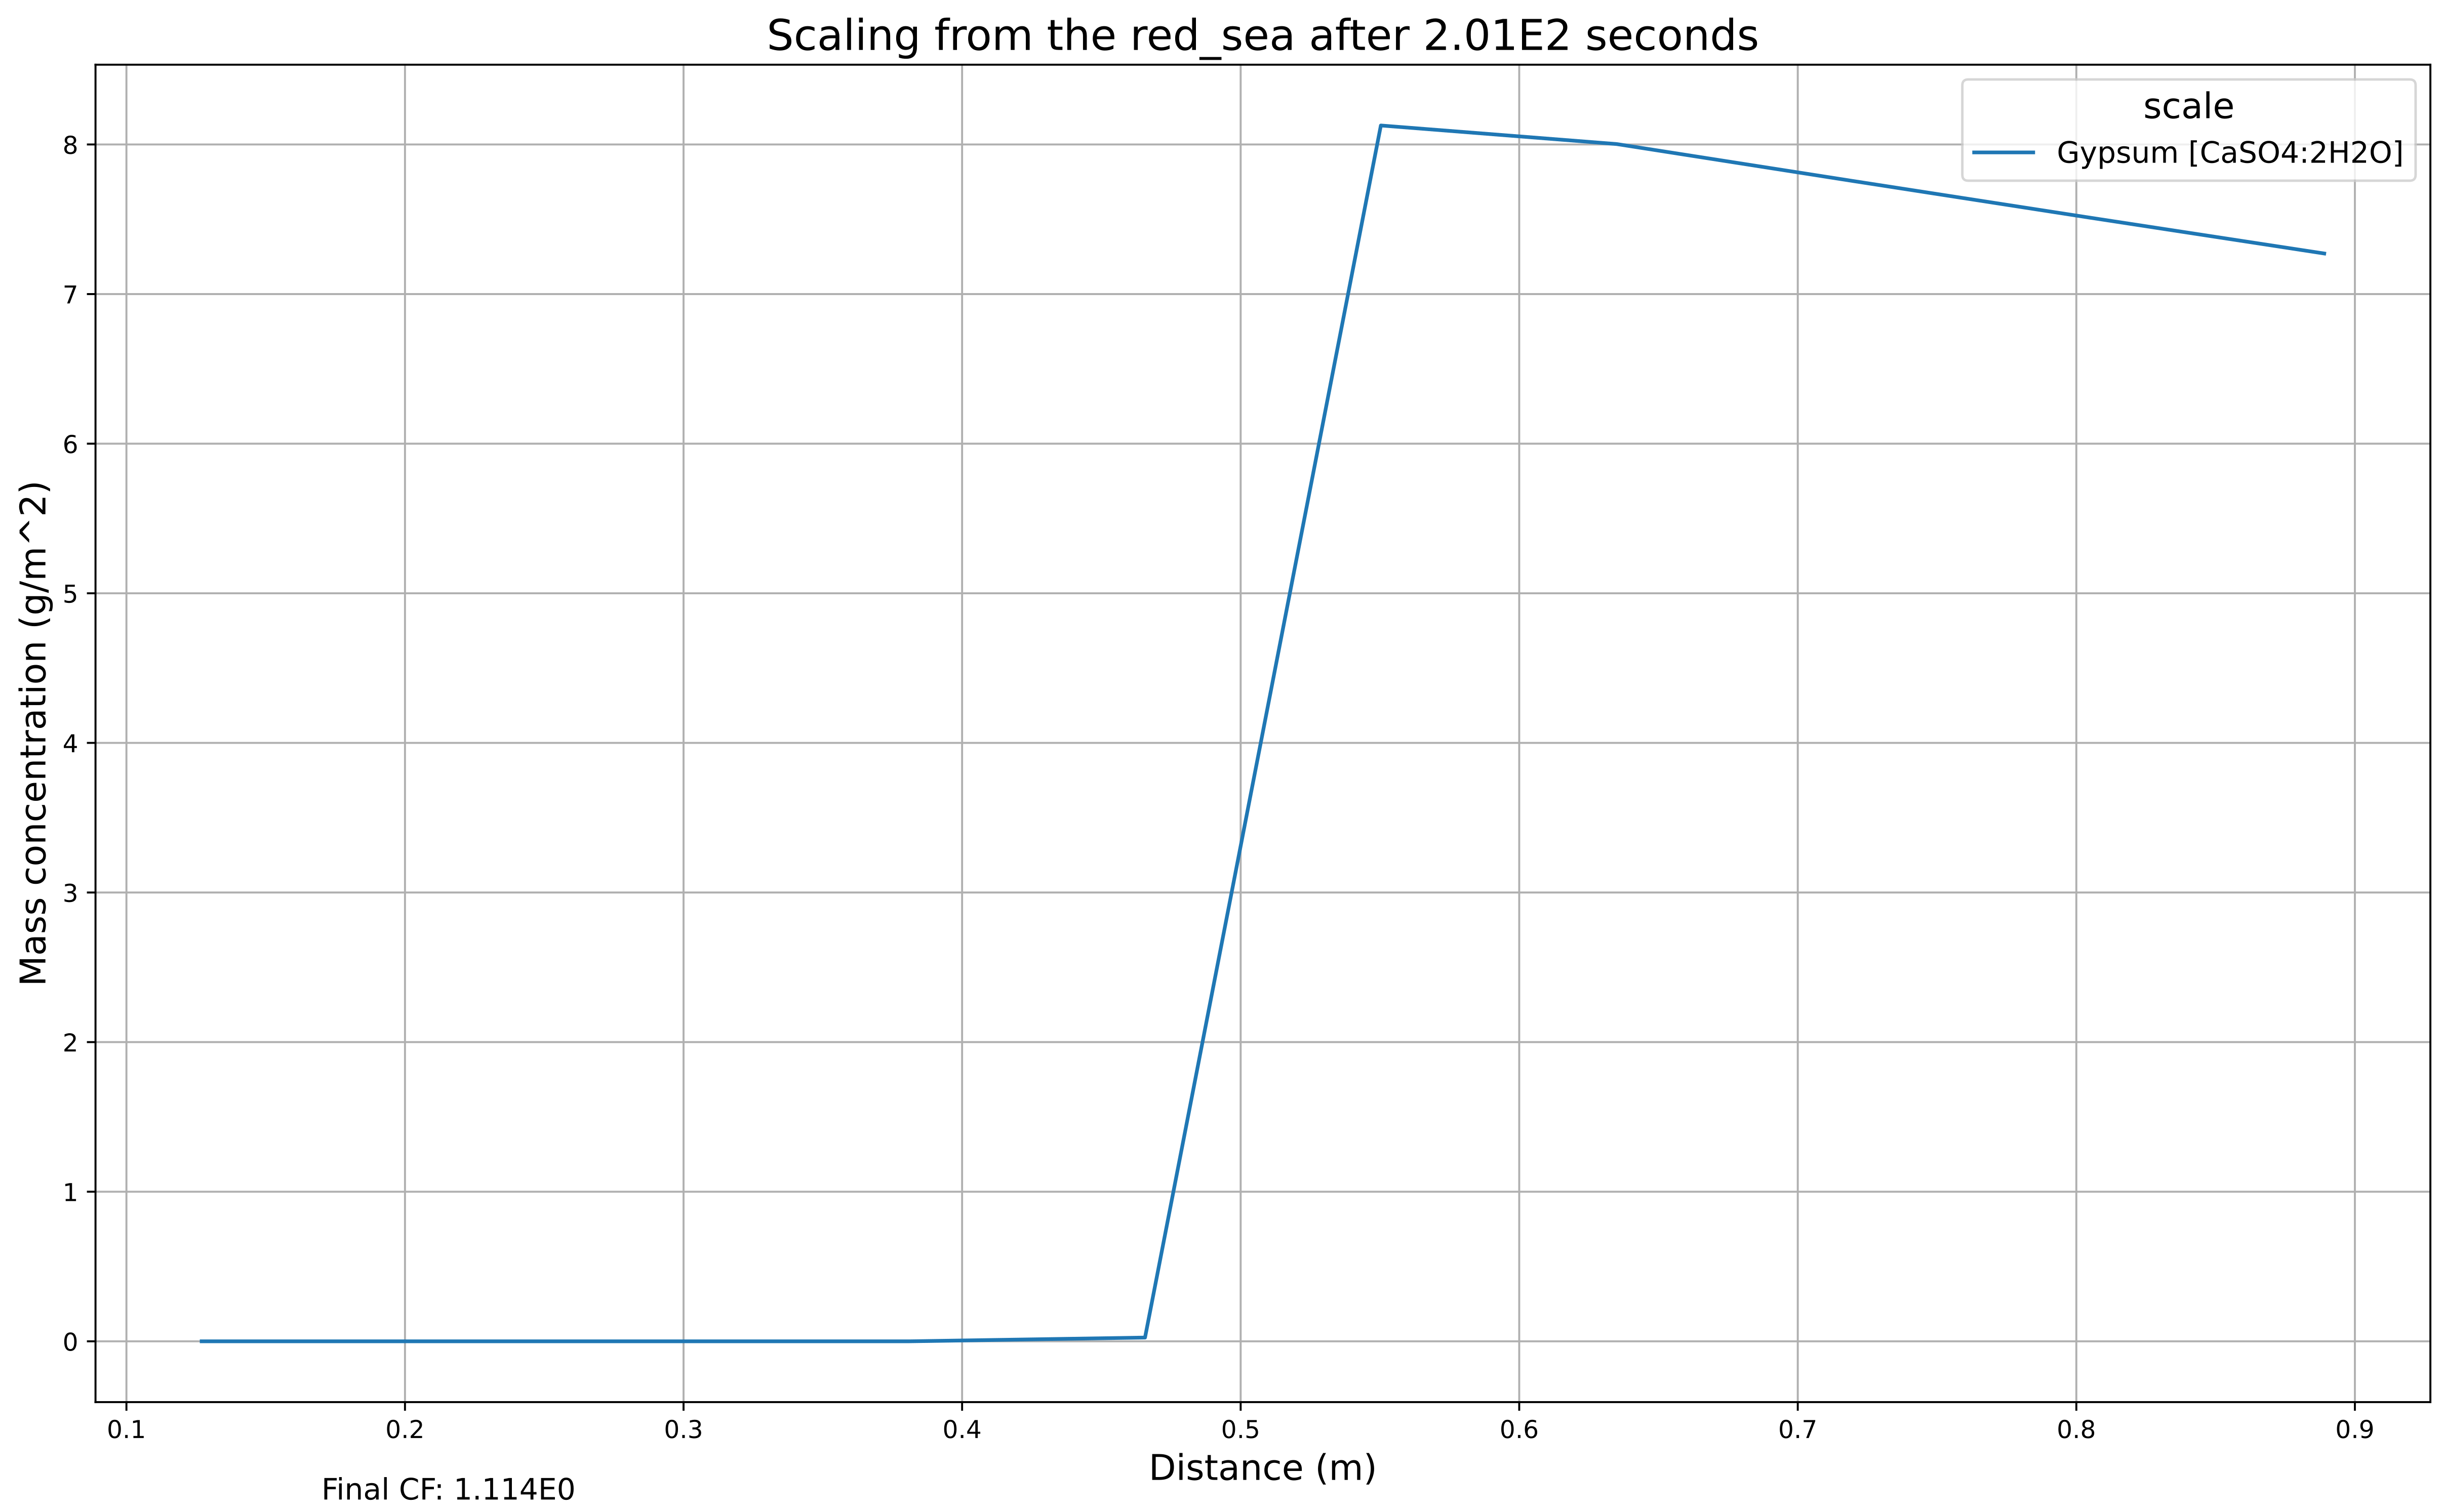
\includegraphics[width=\linewidth]{images/ROSSpy/sensitivity_analyses/evaporation/desalination.png}
    \caption{
        Scaling while a) evaporating and b) desalinating the Red Sea. The two scaling predictions are qualitatively similar, however, even after accounting for the accumulation amongst different pore volumes, the evaporation predictions ($3.36g$) are less than those of the reaction transport simulation ($5.27g$). The difference may be the absence of advection in the evaporation analysis.
    }
    \label{evaporation}
\end{figure}


\subsection{In-series RO arrangements}

In-series arrangements of multiple RO modules are represented by compounding individual modules. We determined that this approach is preferential to a few other methods: e.g. amplifying the characteristics of a single RO module, such as those in Table \ref{RO_dimensions}, by a scalar $r=\frac{\Phi_{\Delta multi-module}}{\Phi_{\Delta module}}$, where the $\Delta \Phi_{multi-module}$ is the total permeate flux of the multi-module system that can be parameterized or approximated through eq. (8). The substitution of $CF_{multi}$ for $CF_e$ and $\Delta \Phi_{multi-module}$ for $\Phi_e$ into eq. (9) permits calculating the $\Delta \Phi_{multi-module}$. 

\begin{savenotes}
\begin{table}[!h]
    \centering
    \begin{tabular}{|c|c|c|}
        \toprule
        \textbf{Parameter} & \textbf{Value} & \textbf{Source} \\ \midrule
        
        \multicolumn{3}{c}{Module (m)} \\ \midrule
        length & 1.016 & BW30-400 \cite{2020FilmTecElement} \\ 
        diameter & 0.201 & BW30-400 \cite{2020FilmTecElement}\\
        permeate tube diameter & 0.029 & BW30-400 \cite{2020FilmTecElement}\\ \midrule
        
        \multicolumn{3}{c}{Membrane (mm)} \\ \midrule
        filtration layer & 0.00025 & \cite{Pacheco2010CharacterizationTechniques,Jeong2007InterfacialMembranes} \\
        Feed spacer & 0.8636 & BW30-400 \cite{2020FilmTecElement} \& \cite{Sablani2002InfluenceSystems} \\
        Permeate spacer & 0.3 & \\
        Polysulphonic layer & 0.05 &  \\
        Support layer & 0.15 &  \\
        Windings $\left( \frac{th_{total}}{th_{membrane}} \right) $ & 86 & BW30-400 \cite{2020FilmTecElement} \\ \midrule
        
        \multicolumn{3}{c}{Membrane cross-section ($m^2$)} \\ \midrule
        Module & 0.0317 & BW30-400 \cite{2020FilmTecElement}\\
        Permeate tube & 0.000661 & BW30-400 \cite{2020FilmTecElement}\\
        Filtration section & 0.0311 & BW30-400 \cite{2020FilmTecElement}\\
        Feed channel & 0.0157 & BW30-400 \cite{2020FilmTecElement}\\ \midrule
        
        \multicolumn{3}{c}{Feed channel capacity} \\ \midrule
        Volume ($m^3$) & 0.0159 & BW30-400 \cite{2020FilmTecElement}\\
        Mass (kg) & 15.86 & BW30-400 \cite{2020FilmTecElement}\\ \midrule

        \multicolumn{3}{c}{Fluid flow ($\frac{m^3}{second}$)} \\ \midrule
        Permeate & 0.000463 & BW30-400 \cite{2020FilmTecElement}\\
        Max Feed & 0.00442 & BW30-400 \cite{2020FilmTecElement}\\ \bottomrule
        
    \end{tabular}
    \caption{
        Default dimensions of an RO module, with corresponding citations, that are primarily based upon the DOW FILMTEC BW30-400 RO module, following precedence from other software \cite{Li2012OptimalDesalination}.
    }
    \label{RO_dimensions}
\end{table}
\end{savenotes}

\subsection{Water bodies}

Additional feed parameter files can be composed by emulating the structure of the default feed parameter files. Literature sources that may foster the development of such feed parameter files for numerous potential feed sources are provided in Table \ref{new_water_bodies} with the respective citations of the experimental geochemical data. 

\begin{table}[h!]
    \centering
    \begin{tabular}{|c|c|}
        \toprule
        \textbf{Water body} & \textbf{Geochemical measurements} \\
        \midrule
        Indian Ocean & \cite{Danielsson1980CadmiumWater,Nisha2014GeochemicalIndia,Stephen-Pichaimani2008EnrichmentIndia,Selvaraj2004EvaluationApproaches,Thangadurai2005Pre-tsunamiIndia,ParvezAl-Usmani2015TraceIndia,Sabine2002InorganicProcesses,Singh2013InternalBengal} \\
        Sargasso Sea & \cite{Bender1976DissolvedSea,Stoffyn-Egli1984MassOceans} \\
        South China Sea & \cite{Calvert1993GeochemistrySeas,Wen2006PhysicochemicalSea,Du2020DynamicsStudy,Chen2001NutrientBasin,Nakaguchi2004DissolvedSea} \\
        Greek Coast & \cite{Chester1981TheSediments,Voutsinou-Taliadouri1983DistributionGreece,Voutsinou-Taliadouri1997DissolvedSeawater} \\
        Toyko Bay & \cite{Fukushima1992TraceJapan} \\
        California Coast & \cite{Hershelman1981MetalsOutfall,Luoma1988DistributionBay,Biller2013SourcesSeason} \\
        North Atlantic & \cite{Loring1978GeochemistryLawrence.,Loring1979GeochemistryLawrence,Yeats1983PotentialAtlantic,Bothner1998MetalTime,Campbell1980BaselineBay,Gaulier2019TraceWaters,Statham1986Dissolved0-35N,Mohamed2011DissolvedOcean,Guay1998ASeas} \\
        Baltic Sea & \cite{Szefer1995DistributionSea,Kremling1978TheStation} \\
        North Pacific & \cite{Tanita2015SurfacePacific,Sim2019Annual20102013} \\
        South Pacific & \cite{Boyle1975CopperZealand,Boyle1976OnCadmium} \\
        General natural waters & \cite{Alibo1999RareOxidation,Klinkhammer1983RareVents,Garcia-Solsona2020RareSea,Longinelli1967Oxygen-18Lakes,Llyod1967Oxygen-18Sulfate,Culkin1966SodiumWater,Krumgalz1982CalciumWaters} \\
        Mississippi Salt Dome Basin & \cite{Kharaka1987GeochemistryU.S.A.} \\
        \bottomrule
    \end{tabular}
    \caption{
        Proposed literature of potential feed water that can be adapted into parameter files for simulation in our model, or specifically ROSSpy.
    }
    \label{new_water_bodies}
\end{table}

\subsection{Dual domain}

\begin{figure}
    \centering
    \begin{tabular}{c|c}
        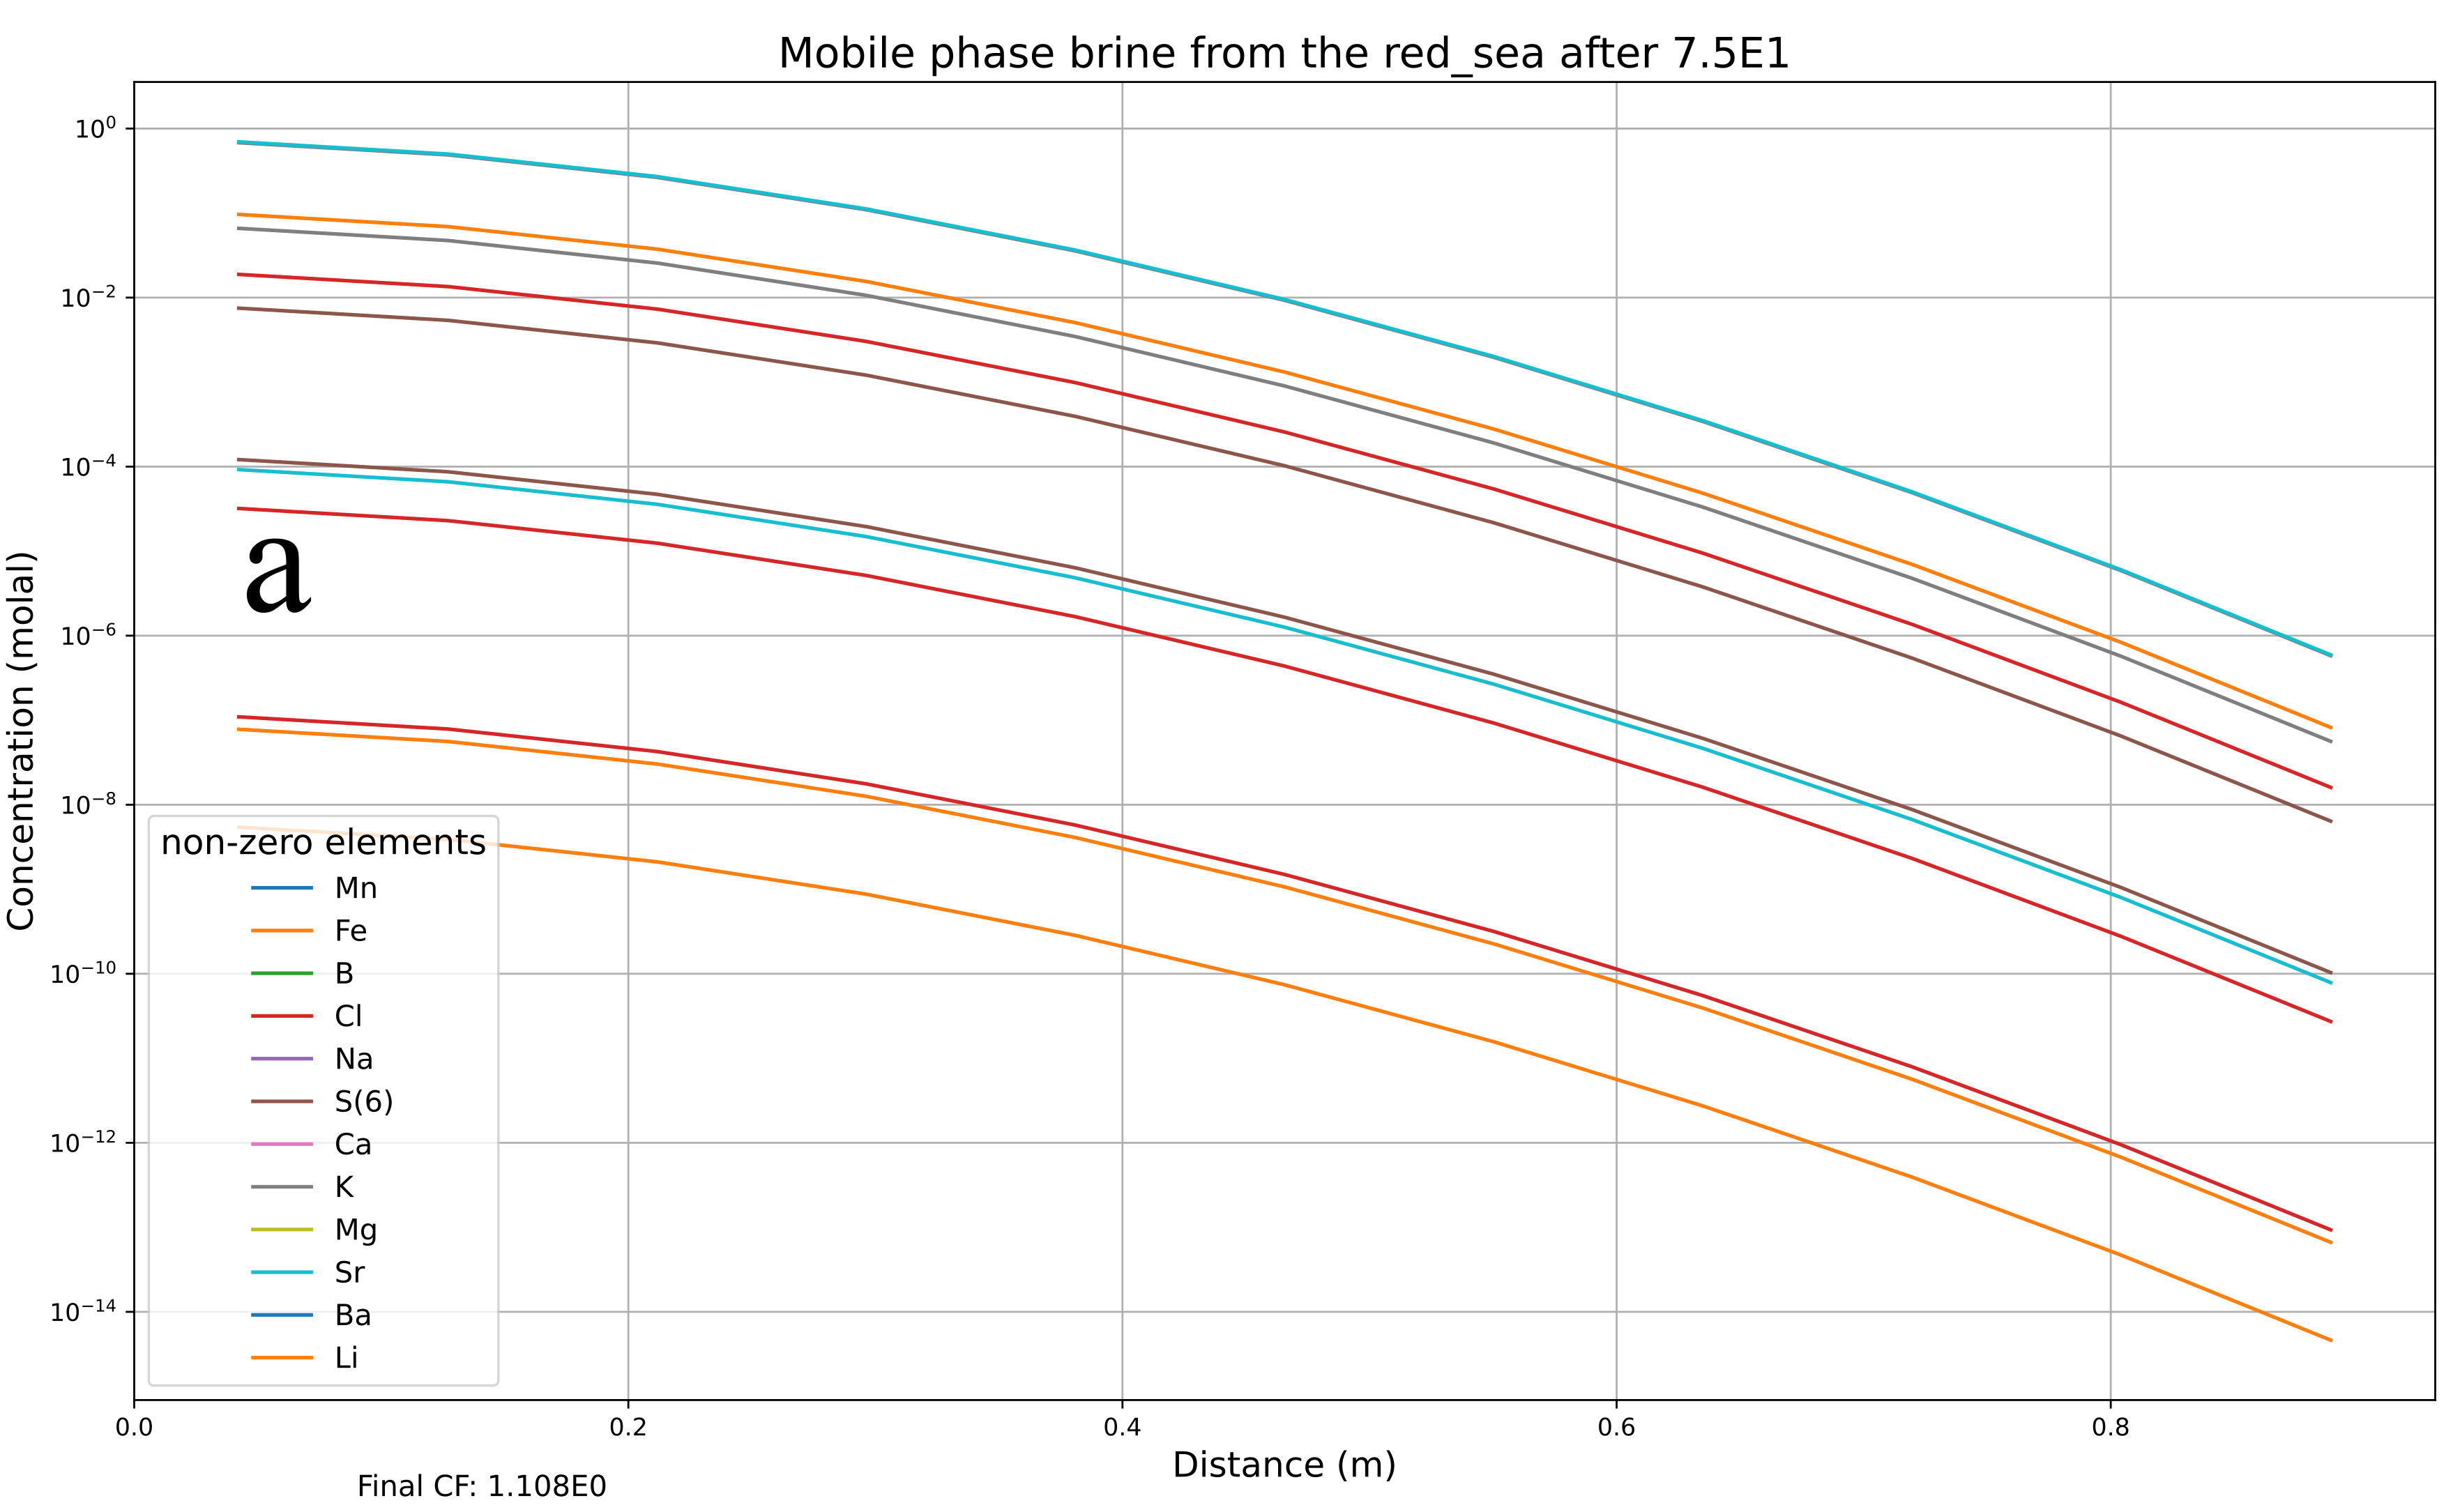
\includegraphics[width=0.49\textwidth]{images/ROSSpy/sensitivity_analyses/EF/mobile_large_ef.png} &
        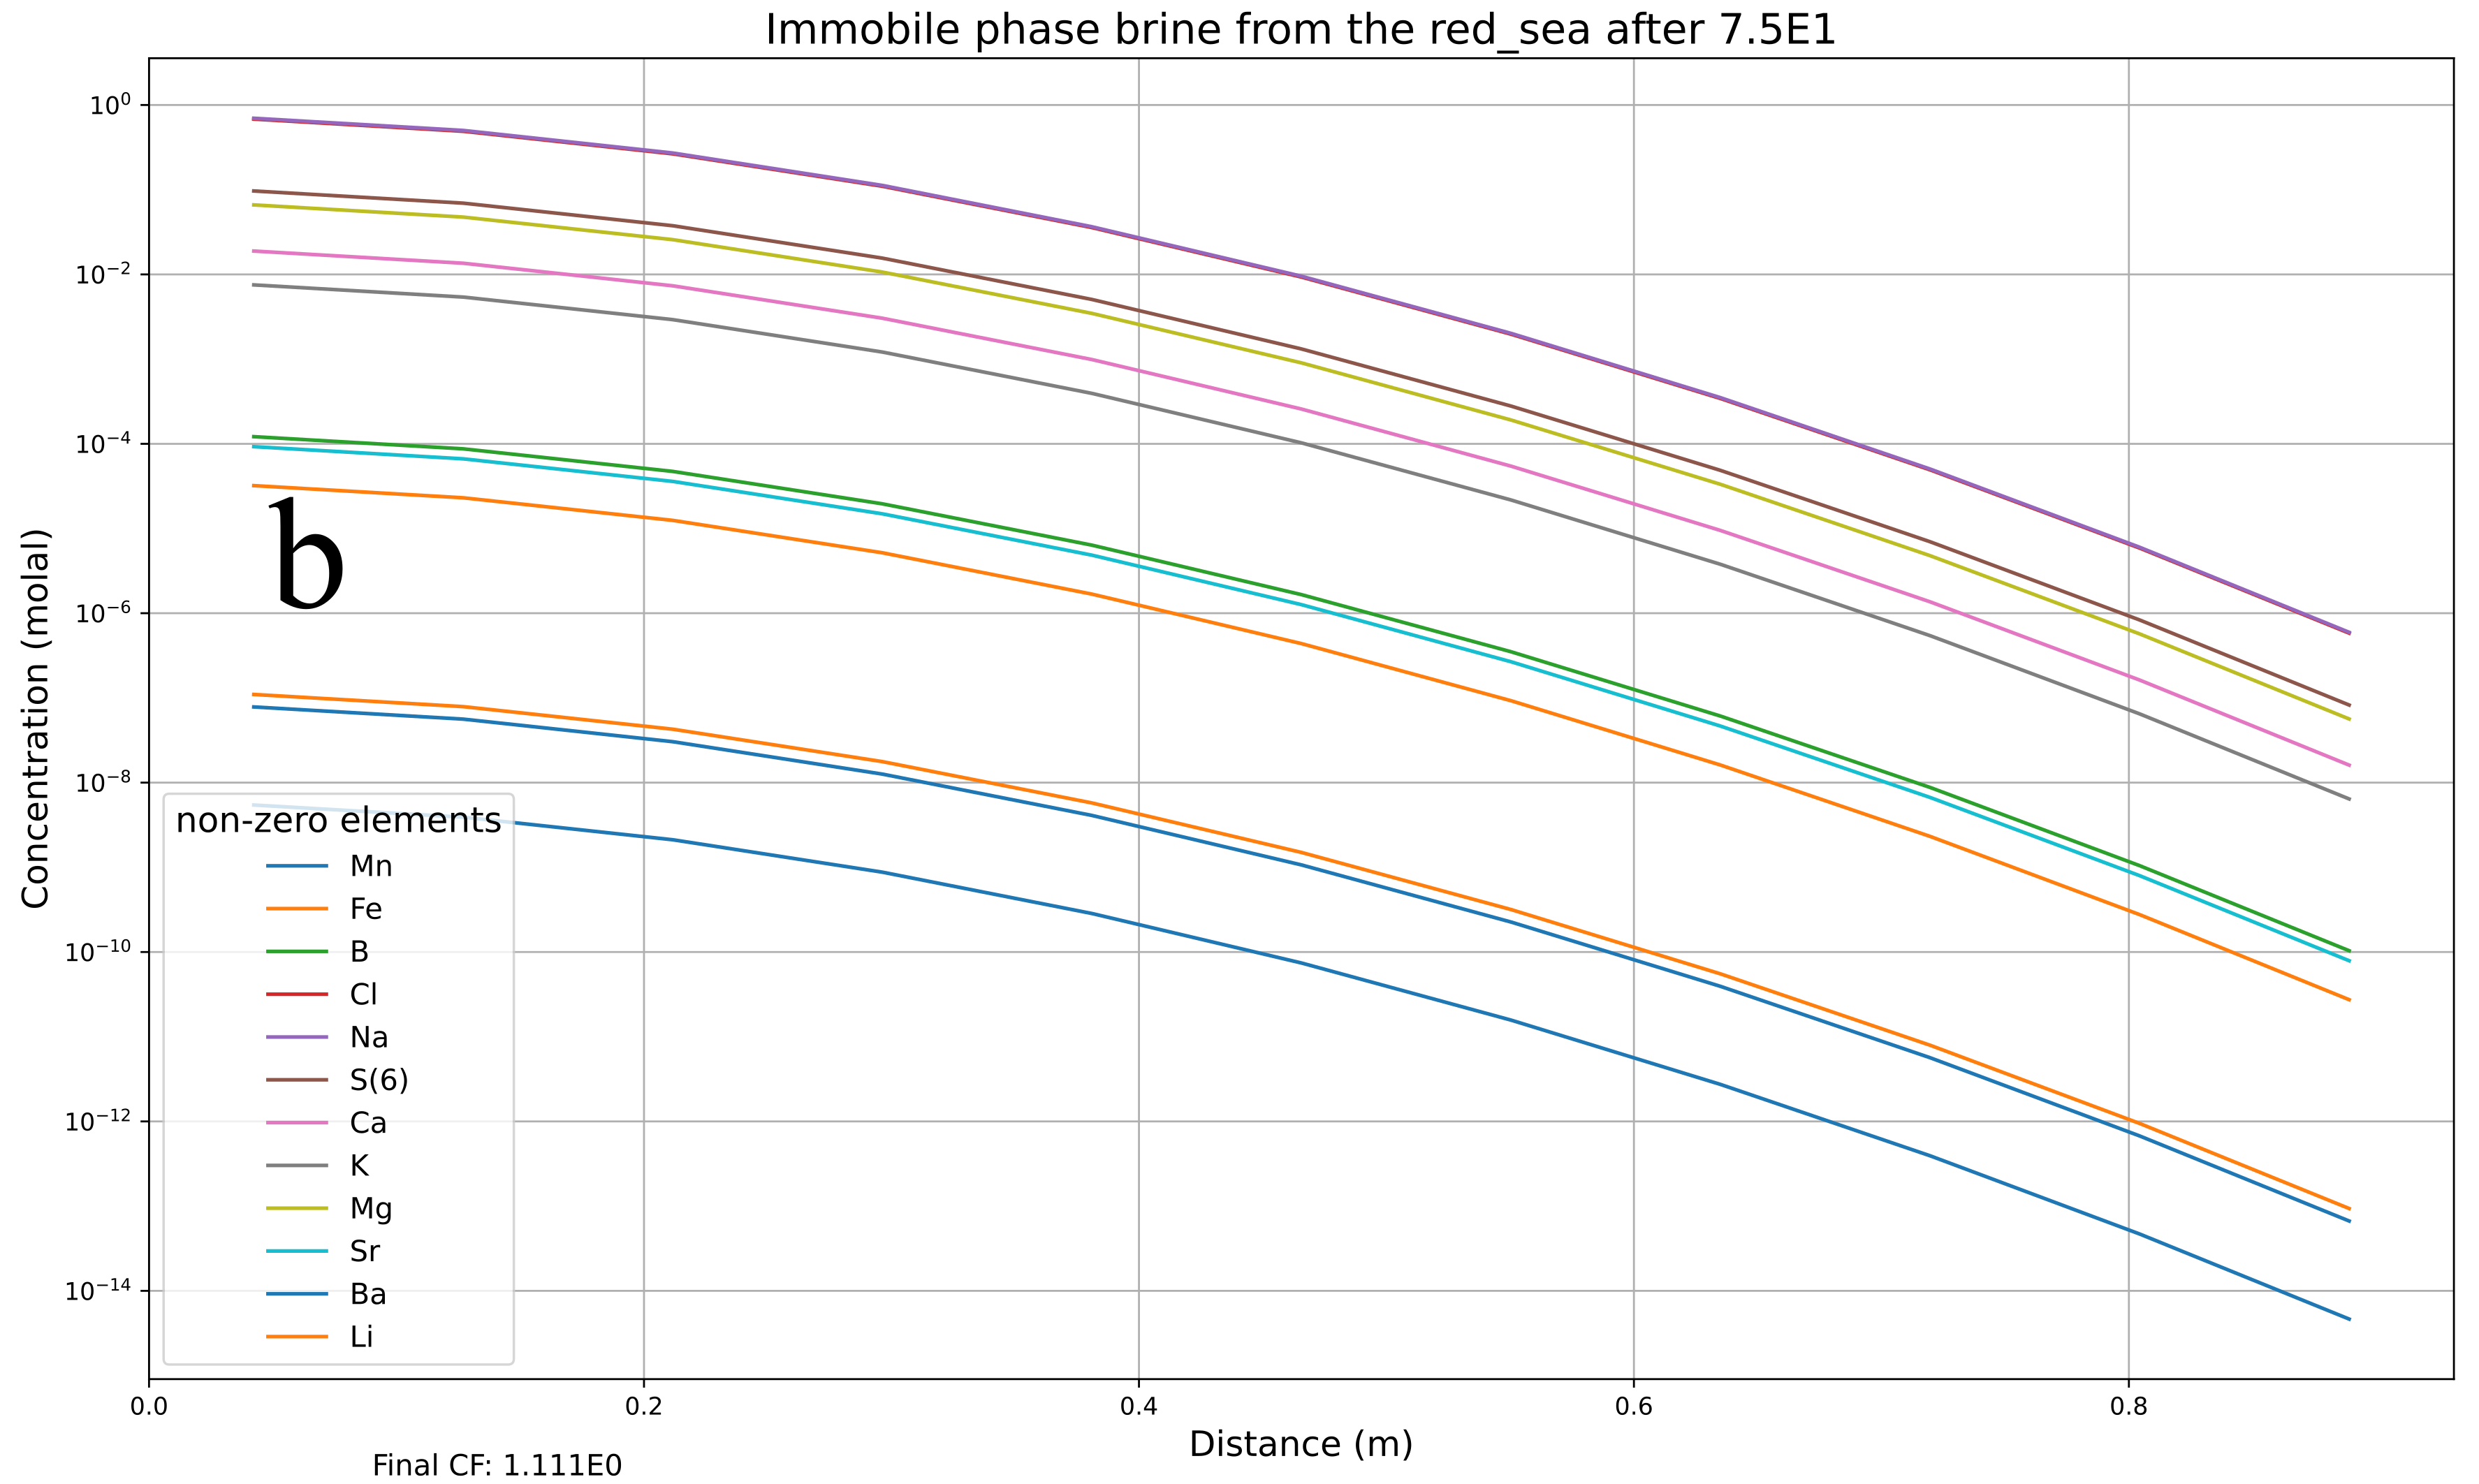
\includegraphics[width=0.49\textwidth]{images/ROSSpy/sensitivity_analyses/EF/immobile_large_ef.png} \\ \midrule
        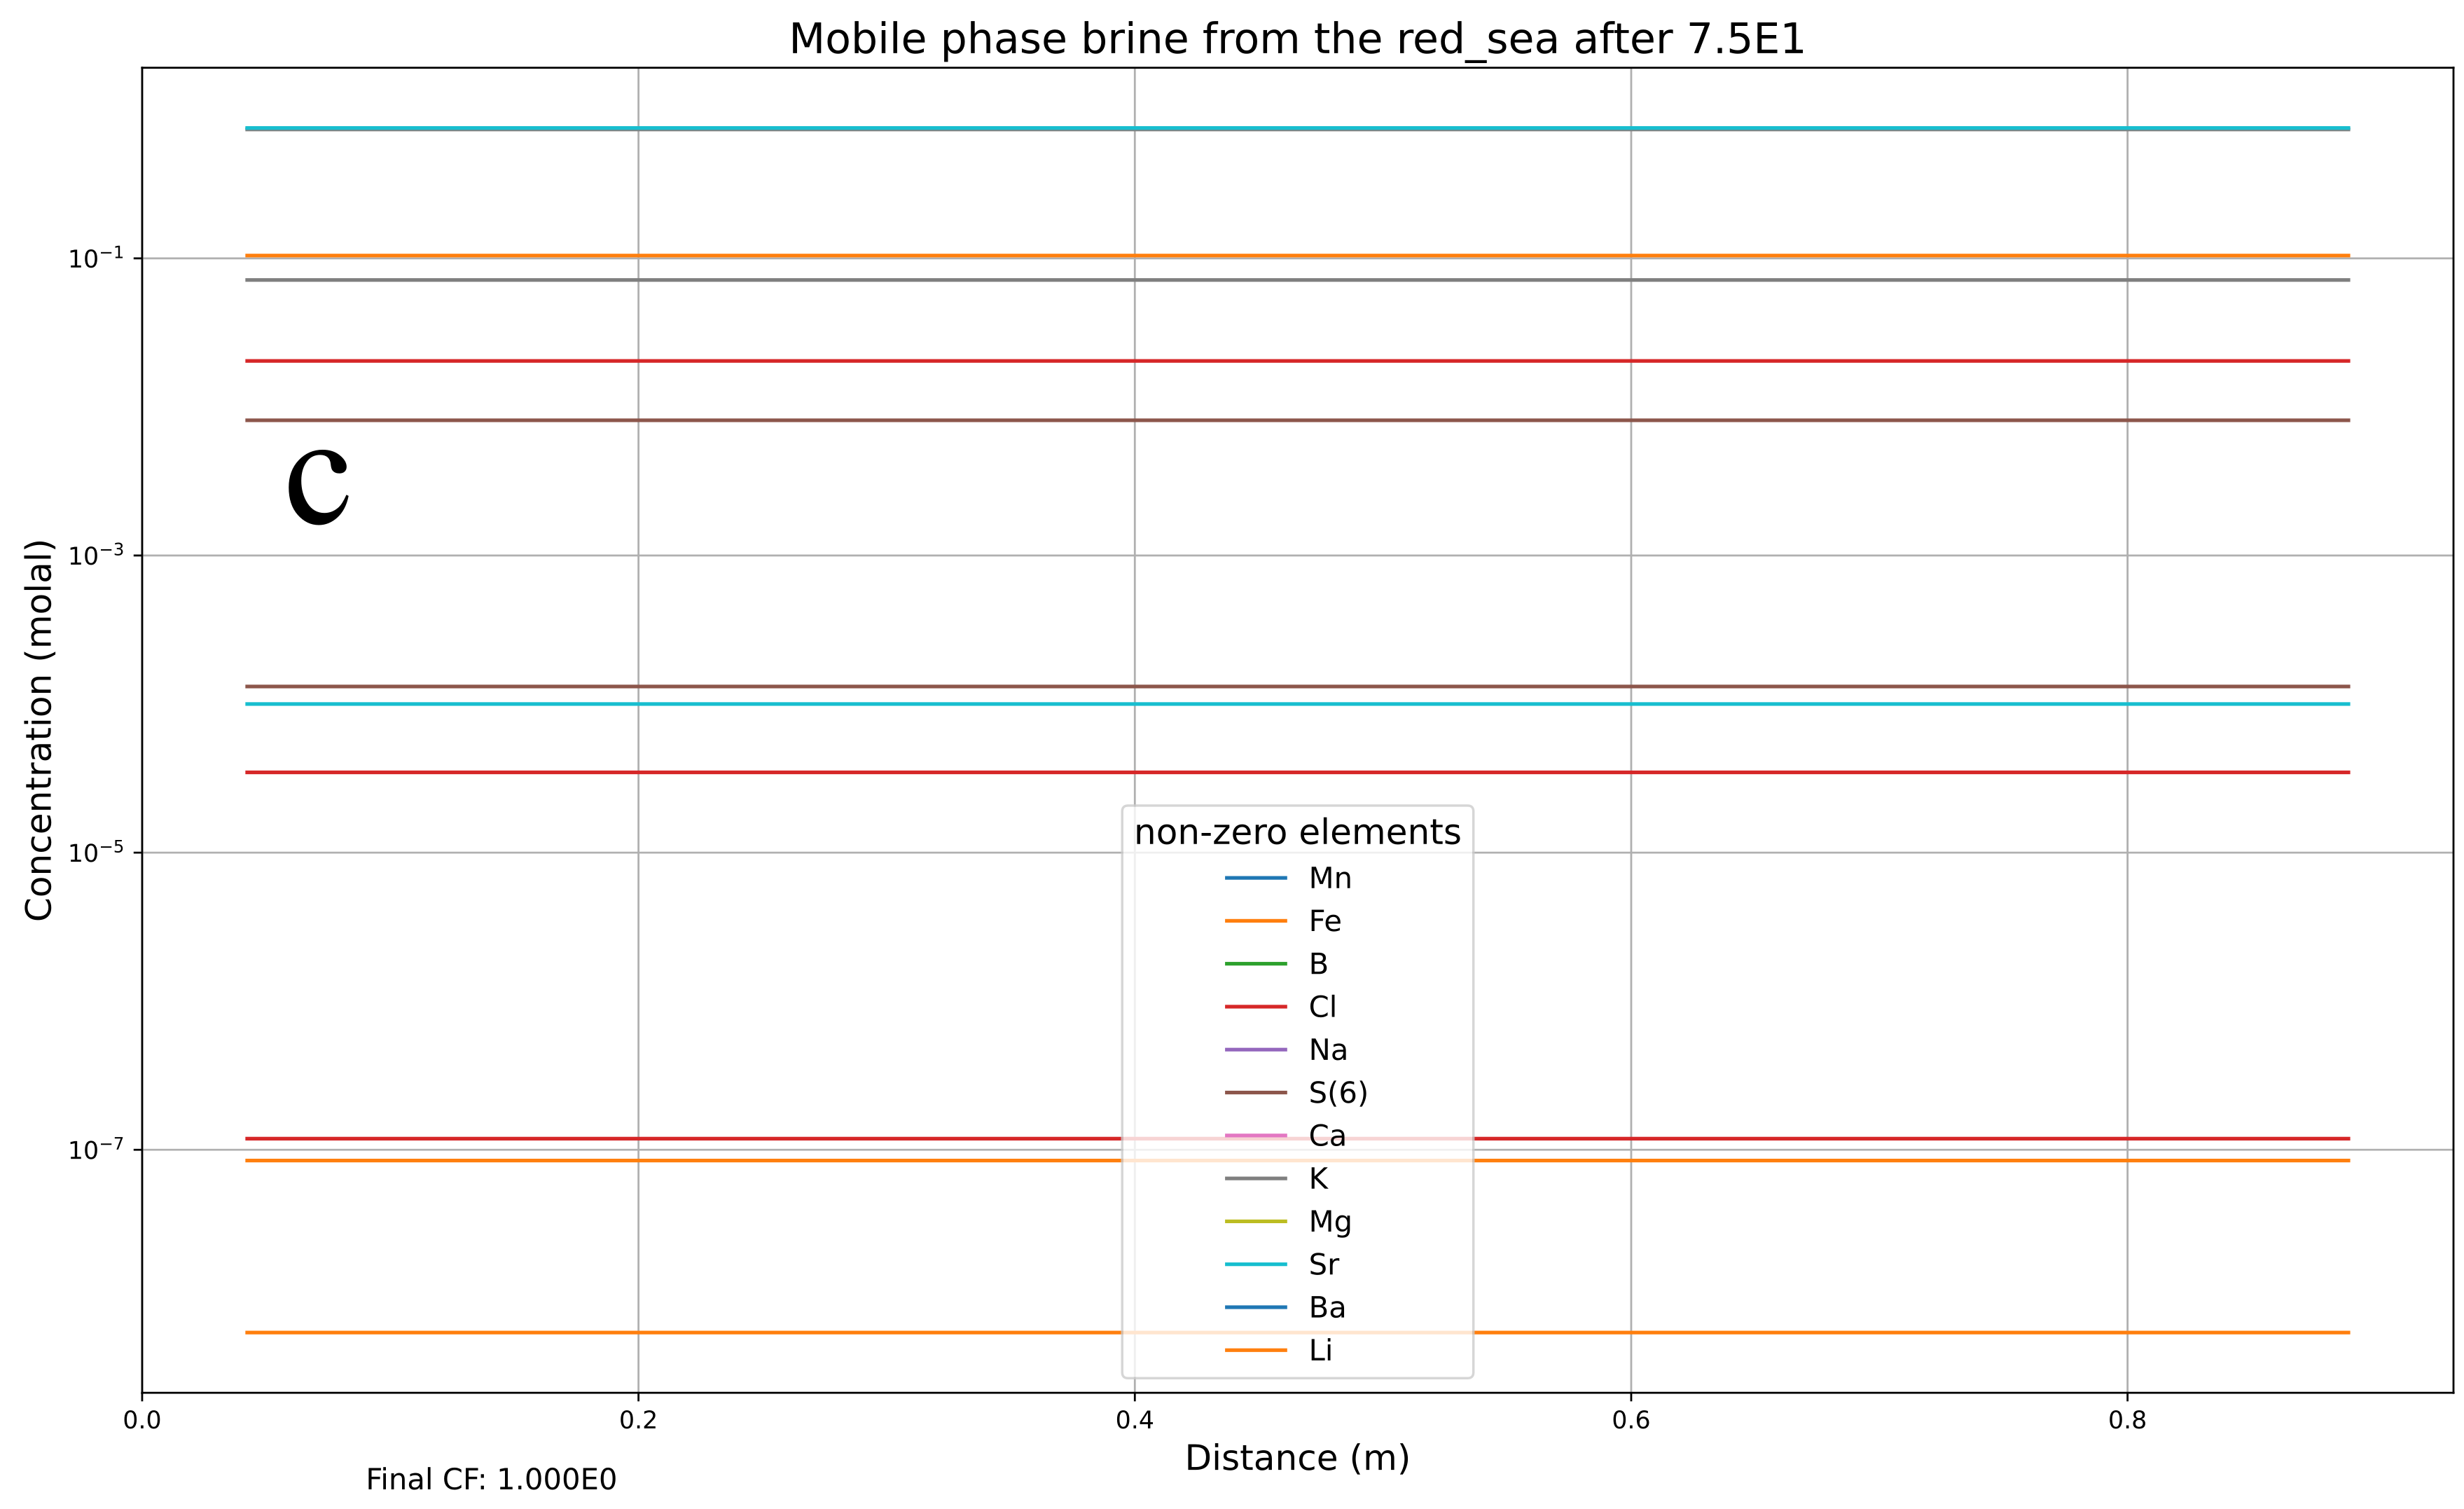
\includegraphics[width=0.49\textwidth]{images/ROSSpy/sensitivity_analyses/EF/mobile_small_ef.png} & 
        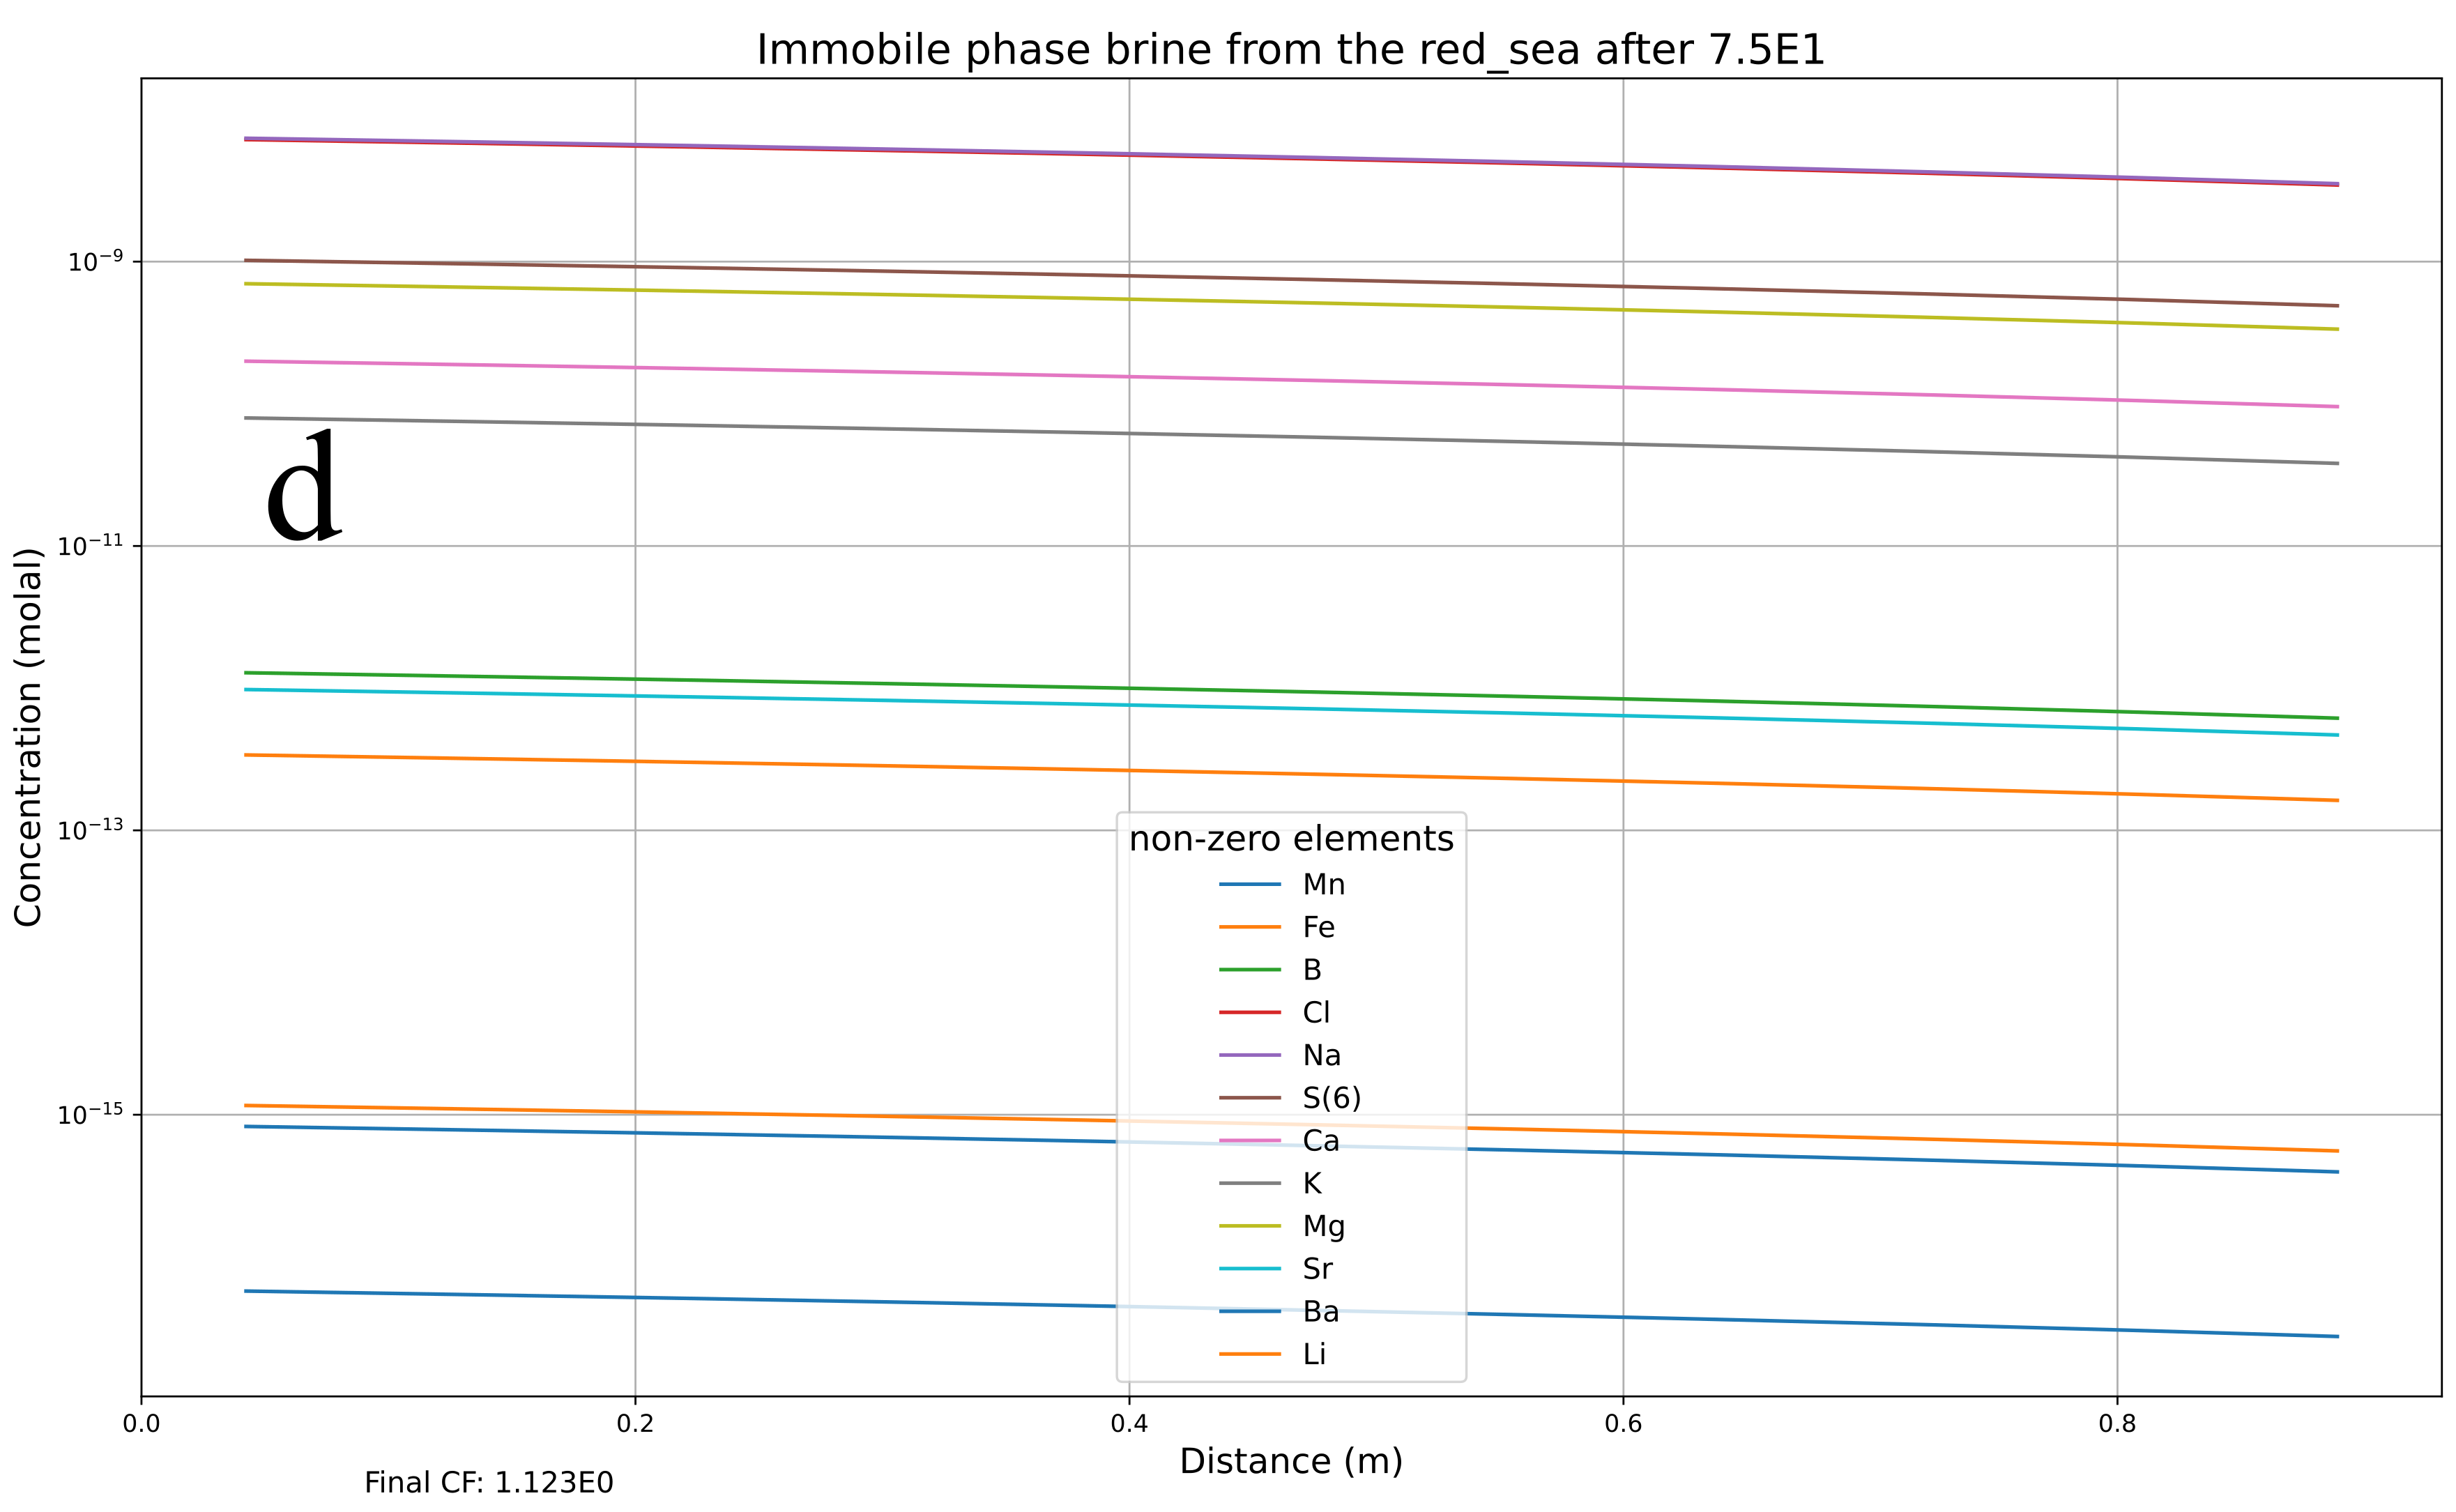
\includegraphics[width=0.49\textwidth]{images/ROSSpy/sensitivity_analyses/EF/immobile_small_ef.png} \\ \bottomrule
    \end{tabular}
    \caption{
        Counter-intuitive brine predictions from dual domain simulations with different exchange factor (EF) values, which is the $\frac{1}{s}$ rate constant of solvent exchange between the mobile and immobile solution phases. Panels a) and b) depict the mobile (bulk) and immobile (CP) phases when $EF=1E10$, while panels c) and d) depict the mobile and immobile phases when $EF=1E-10$, respectively. These non-sensible results motivated our use of the single-domain model to represent RO feed flow. 
    }
    \label{ef_values}
\end{figure}

Our model represents the feed solution with the single-domain model, despite that the dual-domain model in the module cross-section of Figure \ref{single_dual_domain} is more fundamentally accurate, since our attempts to encode the latter in PHREEQC have been unsuccessful. We represent the mobile phase (bulk solution) as one set of membrane cells -- $[1,n]~n\in W$ -- and the immobile phase (CP layer) as a separate set of cells -- $[n+2,m]~m \in W>n+2$. These cell sets exchange solvent at a parameterized rate -- the Exchange Factor $\frac{1}{s}$ (EF) -- which in Figure \ref{ef_values} is very influential upon the simulation predictions; however, the brine concentrations dilute in both solution compartments during desalination simulation. The scaling predictions are equally non-sensible. Our model therefore uses the single-domain model, which appears to be an acceptable approximation per our validations. The developer of PHREEQC -- David Parkhurst -- is uncertain whether the dual-domain model is compatible with the PHREEQ code, which assures us that the single domain model may be the best approximation of desalination reactive transport that is accessible to our open-source framework.

\begin{figure*}
    \centering
    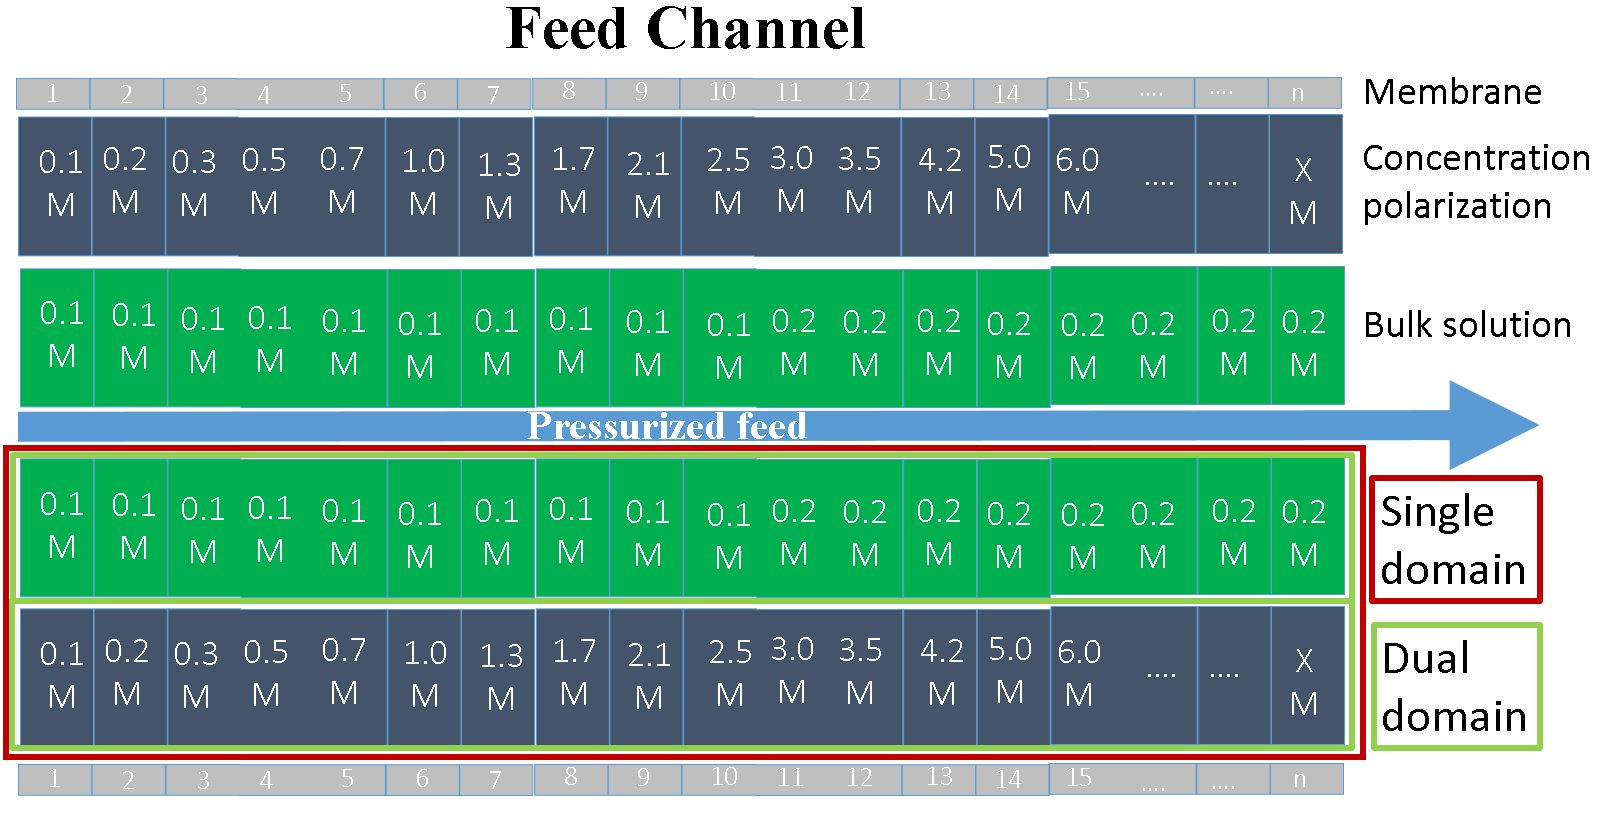
\includegraphics[width = \textwidth]{images/ROSSpy/supporting_information/single_dual_domain.jpg}
    \caption{
        A conceptual cross-section of the RO module. The membrane layers on top and bottom of the figure are discretized into an arbitrary $n$ cells. The figure illustrates the reactive transport phenomena, where the feed solution progressively becomes more concentrated as it transports through the module. The CP layer becomes much more concentrated than the bulk solution as a consequence of the no-slip boundary condition, where the velocity gradient reaches zero at the membrane surface and thus does not diffuse. These bulk and CP solutions are resolved in the dual-domain model (green boxed regions) and are granulated into a single solution by the single-domain model (red boxed regions). The latter was implemented in our model by necessity of PHREEQC.
    }
    \label{single_dual_domain}
\end{figure*}

\subsection{PHREEQ}
The most pertinent calculations of PHREEQC for our model are summarized in the following sub-section, while the version 3 PHREEQC User's manual provides a rigorous description of all PHREEQC operations.

\subsubsection{PHREEQ calculations}
\subsection{PHREEQ calculations}
The total concentration $\Psi_i$ of ionic species $i$ is calculated in each timestep, 
\begin{equation} \label{total_species_concentration}
    \Psi_i=C_i+\sum_{j=1}^{J}(v_{ij}*C_j),
\end{equation}
where $C_i$ is the molal concentration of dissolved $i$; $J$ is the set of compounds that contain $i$; $C_j$ is the molal concentration of compound $j$ that contains $i$; and $v_{ij}$ is the stoichiometric coefficient for the moles of $i$ per mole of compound $j$. The mineral precipitation equilibria over the simulation time $t$ is calculated through a similar equation, 
\begin{equation} \label{concentration_change}
    \frac{\partial \Psi_i}{\partial t}=\sum_{m=1}^{N_m}(v_{mj}*R_m),
\end{equation}
where $N_m$ is the set of reactions that include specie $i$; $v_{mj}$ is the stoichiometric coefficient for the moles of $i$ per mole of mineral $m$; and $R_m$ is the reaction flux of dissolution or precipitation for $(+)$ and $(-)$, respectively,
\begin{equation} \label{mineral_precipitation_reaction}
    R_m=sgn[\Omega]*A_m*k_m*(\Pi(a^n)) |e^{\frac{\eta*\Delta G}{RT}}-1|^p,
\end{equation}
where $\Omega = log\left(⁡\frac{Q_{dissolution}}{K_{sp}}\right)$ and, for the simulated mineral $m$, $A_m$ is the reacting surface area; $k_m$ is the rate constant of dissolution or precipitation; $Q_m$ is the ion activity product constant; and $\eta$ and $p$ are experimentally determined parameters. The $|e^{\frac{\eta * \Delta G}{RT}}-1|^p$ term simplifies to $1$ for irreversible precipitation or dissolution. The set of \cref{total_species_concentration,concentration_change} necessitates that any perturbations to ionic concentrations $\frac{\partial \Psi_i}{\partial t}$ manifest from complexation equilibria. The molal concentration $C_j$ of compound $j$ is discerned,
\begin{equation}
    C_j=\frac{\Pi_{j=1}^{N_c} (\gamma_j*K_j )^{v_{ij}}}{\gamma_j*K_j},
\end{equation}
where $N_c$ is the set of linearly independent chemical reactions; $\gamma_j$ is the activity coefficient of compound $j$; and $K_j$ is the equilibrium constant
\begin{equation}
    K_j=a_j \Pi_m^{M_{aq}} (a_m)^{-v_{m,j}},
\end{equation}
where $M_{aq}$ is the number of minerals in the aqueous system; $v_{m,i}$ is the stoichiometric coefficient of compound $j$ per mole of mineral $m$; and $a_j$ and $a_m$ are the activity coefficients of compound $j$ and mineral $m$, respectively. The activity coefficient $\gamma_j$ is calculated through either the Debye-Hückel model \cite{Aqion2016ActivityModels},
\begin{equation}
    log⁡(\gamma_j)=-A*z_j^2\sqrt{\mu},
\end{equation}
the WATEQ Debye-Hückel model \cite{Aqion2016ActivityModels},
\begin{equation}
    log⁡(\gamma_j)=\frac{-A*z_j^2*\sqrt{\mu}}{1+B*a_j^0*\sqrt{\mu}}+b_j \mu,
\end{equation}
the Davies model \cite{Davies1938TheSulphates},
\begin{equation}
    log⁡(\gamma_j)=-A*z_j^2 (\frac{\sqrt{\mu}}{1+\sqrt{\mu}}-0.2\mu),
\end{equation}
or the empirical Pitzer model \cite{Pitzer1973ThermodynamicsEquations}, where $A$ and $B$ are experimentally determined parameters; $a_j^0$ and $b_j$ are fitted parameters; $z_j$ is the charge of compound $j$; and $\mu$ is the ionic strength of the solution
\begin{equation}
    \mu=\frac{1}{2}\sum_{j=1}^{N_{aq}}z_j^2 \frac{n_j}{W_{aq}},
\end{equation}
where $W_{aq}$ is the simulated water mass and $n_j$ 
\begin{equation}
    n_j=C_j*W_{aq}=\frac{K_i*W_{aq}}{\gamma_j*(\Pi_m^{M_{aq}} (a_m)^{v_{m,j}}}
\end{equation}
is the moles of compound $j$. These calculations and geochemical models are more thoroughly described in the PHREEQC manual and in the cited literature.


\end{supplementary}